\documentclass[12pt]{article}
\usepackage{amssymb,amsmath,times}
\usepackage{color}
\usepackage{graphicx}
\usepackage{fancyhdr}
\usepackage{multirow}
\usepackage{cite}
\usepackage{color}
\usepackage{natbib}
\usepackage{acronym}

% define formatting
%\pagestyle{empty}
\parindent=0pt
\topmargin=0.in \headheight=0in \headsep=-0.1in \textheight=9.2in
\textwidth=6.5in \oddsidemargin=0in

\def\Neff{{N_{\rm eff}}}


% define spacings
\def\p{\smallskip}
\def\sp{\vspace{0.15in}}
\def\spa{\vspace{0.3in}}
\def\spaa{\vspace{0.5in}}
\def\spaaa{\vspace{0.7in}}

% define shorthands for latex commands
\def\bei{\begin{itemize}}
\def\eei{\end{itemize}}

% define commonly used symbols
\def\et{{\it et al.\ }}
\def\degr{$^{\circ}$}
\def\arcsec{$^{\prime\prime}$}
\def\pp{\pi}
\def\Neff{{N_{\rm eff}}}
\newcommand{\hi}{H{\sc i}~}
\newcommand{\HI}{H{\sc i}}


% define various names
\def\usk{ }
\def\max{MAX}
\def\maxima{MAXIMA}
\def\boom{BOOMERanG}
\def\arch{Archeops}
\def\maxboom{\maxima/\boom}
\def\planck{{\it Planck}}
\def\combat{COMBAT}
\def\cmb{CMB}
\def\cmba{CMBA}
\def\tic{Ticra}
\def\codef{CODE5}
\def\forecast{FORECAST}
\def\maxipol{MAXIPOL}
\def\hwp{HWP}
\def\ahwp{AHWP}
\def\wmap{{\it WMAP}}
\def\cobe{{\it COBE}}
\def\igb{IGB}
\def\apex{APEX}
\def\ebex{EBEX}
\def\squid{SQUID}
\def\ld{LD}
\def\ldii{LD-II}
\def\blast{BLAST}
\def\pb{\sc polarbear}
\def\pbsa{{\sc polarbear}/SA}
\def\spttg{SPT3G}
\def\ebextw{EBEX2013}
\def\ebexsk{EBEX-IDS}
\def\litebird{LiteBIRD}
\def\bicep{BKA}
\def\biceptwo{BICEP2}
\def\dfmux{DFMux}
\def\xsixf{$\times$64}
\def\xones{$\times$16}
\newcommand{\core}{\textit{\negthinspace CORE\/}}

% for systematics section
\newcommand{\suffix}{pdf} % for pdflatex
\newcommand{\pico}{PICO}
\newcommand{\prang}{\ensuremath{\alpha}}% Polarisation Rotation Angle
\newcommand{\arcmin}{\ensuremath{'}}
\newcommand{\degree}{\ensuremath{^\circ}}
\newcommand{\fsky}{f_{\rm sky}}
\newcommand{\EFH}[1]{\textcolor{red}{$\dagger${[#1]}$\dagger$}}


%define physics and cosmological notations
\def\het{$^{3}$He}
\def\hef{$^{4}$He}
\def\lnt{lN$_{2}$}
\def\wn{cm$^{-1}$}
\def\omeg{$\Omega$}
\def\omegb{$\Omega_{b}$}
\def\hubble{$H_{0}$}
\def\lamb{$\Lambda$}
\def\cl{$C_{\ell}$}
\def\micron{$\mu$m}
\def\microk{$\mu{\mbox{K}}$}
\def\microkrtsec{$\mu{\mbox{K}}\sqrt{\mbox{sec}}$}
\def\microkamin{$\mu{\mbox{K}}\cdot \mbox{arcmin}$}
\def\microkprthz{$\mu{\mbox{K}}/\sqrt{\mbox{Hz}}$}
\def\wattrthz{${\mbox{Watt}}\sqrt{\mbox{Hz}}$}
\def\voltprthz{${\mbox{Volt}}/\sqrt{\mbox{Hz}}$}
\def\sintheta{\mbox{$\sin\theta$}}
\def\bceti{$\beta$-ceti}
\def\etad{$\eta$-draconis}
\def\ruo2{RuO$_{2}$}
\def\tdot{$\dot{\theta}$}
\def\taub{$\tau_{b}$}
\def\degsq{deg$^2$}

% define polarization symbols parameters
\def\It{$I_{t}$}  
\def\sq{$Q$}
\def\su{$U$}
\def\dsu{$\Delta U$}
\def\dsq{$\Delta Q$}
\def\TT{$C_l^{\rm TT}$}
\def\TE{$C_l^{\rm TE}$}
\def\EE{$C_l^{\rm EE}$}
\def\BB{$C_l^{\rm BB}$}

% define math and vectors

\def\mathrelfun#1#2{\lower3.6pt\vbox{\baselineskip0pt\lineskip.9pt
  \ialign{$\mathsurround=0pt#1\hfil##\hfil$\crcr#2\crcr\sim\crcr}}}
\def\simlt{\mathrel{\mathpalette\mathrelfun <}}
\def\simgt{\mathrel{\mathpalette\mathrelfun >}}

\def\hatx{{\bf \hat n}}
\def\hatnprime{{\bf \hat n'}}
\def\hatnone{{\bf \hat n}_1}
\def\hatntwo{{\bf \hat n}_2}
\def\hatni{{\bf \hat n}_i}
\def\hatnj{{\bf \hat n}_j}
\def\vecx{{\bf x}}
\def\veck{{\bf k}}
\def\hatx{{\bf \hat x}}
\def\hatk{{\bf \hat k}}
\def\hatz{{\bf \hat z}}
\def\VEV#1{{\left\langle #1 \right\rangle}}
\def\cP{{\cal P}}
\def\noise{{\rm noise}}
\def\pix{{\rm pix}}
\def\map{{\rm map}}
\long\def\comment#1{}


%------------------------------------------------------------------------------------------------------
% Tables by Charles Lawrence
%------------------------------------------------------------------------------------------------------
\newbox\tablebox    \newdimen\tablewidth
\def\leaderfil{\leaders\hbox to 5pt{\hss.\hss}\hfil}
\def\endPICOtable{\tablewidth=\wd\tablebox
    $$\hss\copy\tablebox\hss$$
    \vskip-\lastskip\vskip -2pt}
\def\tablenote#1 #2\par{\begingroup \parindent=0.8em
    \abovedisplayshortskip=0pt\belowdisplayshortskip=0pt
    \noindent
    $$\hss\vbox{\hsize\tablewidth \hangindent=\parindent \hangafter=1 \noindent
    \hbox to \parindent{$^#1$\hss}\strut#2\strut\par}\hss$$
    \endgroup}
\def\doubleline{\vskip 3pt\hrule \vskip 1.5pt \hrule \vskip 5pt}
%-------------------------------------------------------------------------------------------------------



% \newcommand{\beq}{\begin{equation}}
% \newcommand{\eeq}{\end{equation}}
% \newcommand{\bea}{\begin{eqnarray}}
% \newcommand{\eea}{\end{eqnarray}}
\newcommand\PRL{{\it Phys.~Rev.~Lett.}}
\newcommand\prl{{\it Phys.~Rev.~Lett.}}
\newcommand\ApJ{{\it Ap.~J.}}
\newcommand\apj{{\it Ap.~J.}}
\newcommand\ApJL{{\it Ap.~J.~Lett.}}
\newcommand\apjl{{\it Ap.~J.~Lett.}}
\newcommand\ApJS{{\it Ap.~J.~Suppl.}}
\newcommand\apjs{{\it Ap.~J.~Suppl.}}
\newcommand\PR{{\it Phys.~Rev.}}
\newcommand\PL{{\it Phys.~Lett.}}
\newcommand\MNRAS{{\it MNRAS}}
\newcommand\mnras{{\it MNRAS}}
\newcommand\MNRASL{{\it MNRAS\ Lett.}}
\newcommand\AnA{{\it Astron.~Astrophys.}}
\newcommand\BAAS{{\it Bull.~Am.~Astron.~Soc.}}
\newcommand\NP{{\it Nucl.~Phys.}}
\newcommand\RMP{{\it Rev.~Mod.~Phys.}}
\newcommand\ARAA{{\it ARAA}}
\newcommand\araa{{\it ARAA}}
\newcommand\prd{{\it Phys.~Rev.~D.}}
\newcommand\plb{{\it Phys.~Lett.~B.}}
\newcommand\ao{{\it Appl.~Optics}}
\newcommand\aap{{\it Astron.~Astrophys.}}
\newcommand\aaps{{\it Astron.~Astrophys.~Suppl.}}
\newcommand\pasp{{\it Proc.~Ast.~Soc.~Pac.}}
\newcommand\josa{{\it J.~Opt.~Soc.~Am.}}
\newcommand\phr{{\it Phys. Reports}}
\newcommand\aj{{\it Astronomical Journal}}
\newcommand\jcap{{\it JCAP}}
\newcommand\apss{{\it ApSS}}
\newcommand\nat{{\it Nature}}
\newcommand\procspie{{\it Proceedings of SPIE}}
\newcommand\pasj{{\it Publications of the Astronomical Society of Japan}}
\newcommand\ssr{{\it Space Science Reviews}}
\newcommand\physrep{{\it Physics Reports}}
\newcommand\aapr{{\it Astronomy and Astrophysics Review}}
\newcommand\nar{{\it New Astronomy Reviews}}


\newcommand{\comred}[1]{\textcolor{red}{#1}}
\newcommand{\comblue}[1]{\textcolor{blue}{#1}}
\newcommand{\comgreen}[1]{\textcolor{green}{#1}}
\newcommand{\comor}[1]{\textcolor{orange}{#1}}

\newcommand{\sored}[1]{\comred{\sout{#1}}}
\newcommand{\soor}[1]{\comor{\sout{#1}}}

% Let's you define a command for both text and math mode. 
\newcommand{\wisk}[1]{{\ifmmode{#1}\else{$#1$}\fi}}






\setlength{\floatsep}{0.5\floatsep}
\setlength{\textfloatsep}{0.5\textfloatsep}
\setlength{\intextsep}{0.5\intextsep}
\setlength{\floatsep}{0.5\floatsep}
\setlength{\dblfloatsep}{0.5\dblfloatsep}
\setlength{\dbltextfloatsep}{0.5\dbltextfloatsep}

\begin{document}

\bibliographystyle{unsrt}

\setlength{\baselineskip}{0.96\baselineskip} %% measured, 5.0 lines/inch.  Can go to 0.96\baselineskip
\setlength{\parskip}{1.\parskip}

\parindent = 15pt

\tableofcontents

\setcounter{page}{0}
\setcounter{figure}{0}

\newpage
%\twocolumn

\section{Executive Summary (1 pg)} 
\documentclass[PICOReport.tex]{subfiles}

\begin{document}

%% Beginning of Martin

The \ac{CMB} comes to us from the furthest reaches of the observable Universe, and its photons experience all of cosmic history.  Created when the Universe was a hotter, simpler place, CMB photons carry information about fundamental physics, the constituents of the cosmos, and the theory of gravity.  On their journey they feel the impact of the gravitational potentials formed by the cosmic web of superclusters, clusters, and galaxies.  They interact with the ionized gas in the inter- and circum-galactic media, gas that eventually fuels star and galaxy formation.  Superposed upon the CMB is the emission from multiple extragalactic sources and from our Galaxy.  All of this leaves an imprint that sensitive measurements can disentangle so that CMB studies impact every aspect of cosmology and many areas of astrophysics.

%The \ac{CMB} comes to us from the furthest reaches of the observable Universe, and its photons experience all of cosmic history.  Created when the Universe was a hotter, simpler place, CMB photons probe fundamental physics, provide exquisite measurements of the constituents of the cosmos, and test relativity.  On their journey they feel the impact of the gravitational potentials formed by the cosmic web of superclusters, clusters, and galaxies.  They interact with the ionized gas in the inter- and circum-galactic media, gas that eventually fuels star and galaxy formation.  Superposed upon the CMB is the emission from multiple extragalactic sources and from our Galaxy.  All of this leaves an imprint that sensitive measurements can disentangle so that CMB studies impact every aspect of cosmology and many areas of astrophysics.

\begin{wrapfigure}{R}{0.31\textwidth}  % r is right aligned, l is left. Capital letters allow figure to float on page.
\vspace{-5pt} % if move up and reduce to 12 lines only (add [12] before {R}) saves 1 line.
\includegraphics[width=0.31\textwidth]{images/PICO_Image.jpg}
\vspace{-0.25in}
\caption{\captiontext The PICO spacecraft 
\label{fig:pico_rendered} }
\end{wrapfigure}

Building upon a legacy of successful measurements, the next decade holds tremendous potential for new, exciting \ac{CMB} discoveries, to be delivered by the Probe of Inflation and Cosmic Origins (PICO, Fig.~\ref{fig:pico_rendered}). PICO is an imaging polarimeter that will scan the sky for 5 years in 21 frequency bands spread between 21 and 799~GHz; see Tables~\ref{tab:specs} and \ref{tab:spec_bands}. It will produce %ten independent 
full-sky surveys of intensity and polarization with a final combined-map noise level equivalent to 3300 \planck\ missions for the baseline required specifications, and according to our current best-estimate would perform as 6400 \planck\ missions.  

With these capabilities, unmatched by any other existing or proposed platform, PICO will address seven science objectives (SOs), which are listed in Table~\ref{tab:STM}. Delivering this set was the basis for selecting PICO's design and for setting instrument requirements. But, as described in this report, PICO's science reach is broader than the baseline set. 

PICO could determine the energy scale of inflation and give a first, direct probe of quantum gravity (SO1). %, \S~\ref{sec:fundamentalsci}). 
The mission will attempt to detect the signal that arises from gravitational waves sourced by inflation and parameterized by the tensor-to-scalar ratio $r$ at a level of $r =5\times10^{-4} \, (5\sigma)$. This level is 100 times lower than current upper limits, and more than 10 times lower than limits forecast by funded future experiments.  If the signal is not detected, PICO will constrain broad classes of inflationary models, exclude at $5 \sigma$ models for which the characteristic scale in the potential is the Planck scale, and distinguish between reheating scenarios at $3\sigma$ (SO1 and SO2). The combination of data from PICO and LSST could rule out all models of slow-roll single-field inflation, marking a watershed in studies of inflation. 
%If the signal is not detected, PICO will constrain broad classes of inflationary models and exclude at $5 \sigma$ models for which the characteristic scale in the potential is the Planck scale (SO1 and SO2). The combination of data from PICO and LSST can constrain features in the inflationary potential, the field content during inflation and could rule out all models of slow-roll single-field inflation, marking a watershed in studies of inflation. \comor{reword?}


The mission will have a deep impact on particle physics by measuring the minimum expected sum of the neutrino masses with $4\sigma$ confidence, rising to $7\sigma$ if the sum is near 0.1~eV (SO3). Reaching the $4\sigma$ level can only be achieved with an instrument that can measure the polarization of the CMB on the largest angular scales, a measurement best done from space, which gives access to the full sky, and with a broad band of frequencies to remove foreground contaminants.  
Cluster counts provided by PICO in combination with followup redshift measurements, and PICO's map of the projected gravitational potentials along the line of sight in combination with the LSST gold sample of galaxies, will give two additional independent and equally competitive constraints on the sum of neutrino masses. 

The measurements will either detect or strongly constrain deviations from the standard model of particle physics by counting the number of light particle species $N_{\rm eff}$ in the early universe.  The constraint of $\Delta N_{\rm eff} < 0.06 \, (2\sigma)$ will move the allowed decoupling temperature of a hypothetical new vector particle to temperatures that are 400 times higher than currently determined by \planck\ (SO4). The data will constrain generic models of dark matter, and enable a search for primordial magnetic fields with sufficient sensitivity: to rule them out as the sole source for the largest observed galactic magnetic fields; and to improve by a factor of 300 constraints on polarization rotation arising from early Universe fields that lead to cosmic birefringence, and thus constrain string theory-motivated axions. 

PICO will elucidate the processes affecting the evolution of cosmic structures. It will measure the optical depth to reionization $\tau$ with an error $\sigma(\tau) = 0.002$, limited only by the small number of spatial modes available in the largest angular scale CMB polarization (SO5). The measurement will be used to constrain models of the formation of the first luminous sources, and is a key input to all astrophysical attempts to improve the determination of the sum of neutrino masses. The data will give a map of the projected gravitational potential due to all structures with a \ac{SNR} 14 times higher than \planck , and a catalog of 150,000 clusters extending to their earliest formation redshift. Each of these datasets will be used in combination with other data -- from LSST and from future optical and infrared surveys -- to independently constrain the evolution of the amplitude of linear fluctuations $\sigma_{8}(z)$, with sub-percent accuracy.  

Cross-correlating PICO's map of the thermal Sunyaev--Zeldovich effect with LSST's gold sample of galaxies, a correlation that is forecast to have a \ac{SNR} exceeding 1000, will give precise tracing of the evolution of thermal pressure with $z$. This will be used to place constraints on models of baryonic feedback, which is the most uncertain ingredient in models of galaxy formation. 

%Galactic emissions which act as foregrounds and are stronger than the CMB polarized intensity will be separated using PICOs 21 bands spread over a broad frequency bandwidth. 

$\Lambda$CDM provides a good fit to most current data with only six parameters. But the model leaves fundamental questions open. Premier among them is the unknown content of the majority of the Universe. PICO data will reduce the allowed volume of uncertainty in a 12-dimensional $ \Lambda$CDM parameter space by a factor of nearly a billion relative to current \planck\ constraints. Such exquisite scrutiny of the prevailing paradigm will either give strong validation or require yet-to-be discovered revisions.

PICO's maps of the Milky Way will be used to resolve long-standing questions about our own Galaxy. Galactic interstellar dust grains are a link between atoms and molecules and planetary objects, yet their composition and their role in Galactic chemistry is still under debate. Galactic magnetic fields are known to play a key role in the dynamics of gas in the Galaxy, and in determining the efficiency of star formation, but their quantitative contribution relative to turbulence is yet to be determined. With the mission's Galactic dust polarization maps we will constrain dust properties, including composition, temperature, and emissivities (SO6), and we will make maps of the Galactic magnetic field. These detailed 1\arcmin\ resolution maps will be used to quantify the relative roles of gas turbulence and magnetic fields in the dynamics of the Galaxy and in the observed low star-formation efficiency (SO7). 

PICO will give deep, full-sky legacy maps with which astrophysicists will constrain the early phases of galaxy evolution by discovering 4500 strongly lensed dusty galaxies with $z$ up to 5; investigate the early phases of cluster evolution by discovering 50,000 proto-clusters out to $z\sim4.5$; perform a census of cold dust in 30,000 low $z$ galaxies; make cosmic infrared background maps of the anisotropies due to dusty star-forming galaxies; map magnetic fields in 70 nearby galaxies; and, with a 3,000-fold increase relative to \planck\ in the number of independent measurements of magnetic field in our own Galaxy, study how magnetic fields are generated through a combination of turbulence and large-scale gas motion. This rich harvest will be contained in maps of both intensity and polarization at 21 frequency bands, each much more sensitive than \planck 's nine frequency maps in intensity and seven in polarization. At 30, 155, and 385~GHz PICO's noise is 17, 40, and 100 times lower than \planck 's at 30, 143, and 353~GHz, respectively. Six of the PICO maps in bands between 321 and 800~GHz, which are key for the high $z$ science, are not accessible to ground-based instruments; \planck\ did not have polarization information above 353~GHz and PICO's highest resolution is five times finer than \planck 's. Only a space mission like PICO will provide such full-sky legacy maps. 


%Five of the PICO bands between 385 and 800~GHz are key for the high $z$ science; \planck\ did not have polarization information above 353~GHz and PICO's highest resolution is five times finer than \planck 's. Only a space mission like PICO will provide such full-sky legacy maps. 


%PICO will give full-sky maps of intensity and polarization at 21 frequency bands, each much more sensitive than \planck 's nine frequency maps in intensity and seven in polarization. At 30, 155, and 385~GHz PICO's noise is 17, 40, and 100 times lower than \planck 's at 30, 143, and 353~GHz, respectively. Five PICO bands will have polarization information at frequencies between 385 and 800~GHz that \planck\ did not have, and PICO's highest resolution is five times finer than \planck 's. Only PICO will provide such full-sky legacy maps. With the six maps at frequencies not accessible to ground-based experiments we will: constrain the early phases of galaxy evolution by discovering 4500 strongly lensed dusty galaxies with $z$ up to 5; investigate the early phases of cluster evolution by discovering 50,000 proto-clusters out to $z\sim4.5$; perform a census of cold dust in 30,000 low $z$ galaxies; make cosmic infrared background maps of the anisotropies due to dusty star-forming galaxies; map magnetic fields in 70 nearby galaxies; and, with 3,000-fold increase relative to \planck\ in the number of independent measurements of magnetic field in our own Galaxy, study how magnetic fields are generated through a combination of turbulence and large-scale gas motion. 

With its broad frequency coverage, PICO is better equipped than any other current or planned instrument to separate the detected signals into their original sources of emission.  This capability is most important for unveiling the faintest of signals, the telltale signature of inflation, which is already known to be dominated by Galactic foregrounds. Our simulations indicate that PICO's combination of low noise and multitude of bands is sufficient to separate the inflationary signal from the foregrounds at the required level. But there are uncertainties in the modeling of Galactic foregrounds. To reduce these uncertainties and gain further confidence we recommend support for: (1) modeling, simulation, and algorithm development for effective foreground separation; and (2) improved Galactic emission measurements with sub-orbital experiments. 

%With its broad frequency coverage PICO is better equipped than any other current or planned instrument to separate the detected signals to their original sources of emission.  This capability is most important for the faintest of signals, the telltale of inflation, which is already known to be dominated by Galactic foregrounds. Our simulations indicate that PICO's combination of low noise and multitude of bands is sufficient to separate the inflationary signal from the foregrounds at the required level. But current uncertainties on the parameters characterizing Galactic foregrounds are large and we recommend support for (1) modeling, simulation, and algorithm development for effective foreground separation, and (2) improved Galactic emission measurements with sub-orbital experiments. 
%\comor{combine recommendations}?

% [TJP] ------------------------
% [TJP] The Science Traceability Matrix goes here. The table is in stm.tex, but the following LaTeX invocation makes it appear on a double-wide page
\afterpage{%
  % switch to LayoutPageB (includes switching page size)
  \switchToLayoutPageB{}
    \input stm.tex
   \clearpage
% start with LayoutPageA (includes switching page size)
\switchToLayoutPageA{}
% \input stm2.tex  stm2 moved to Legacy science section. (Karl)
% \clearpage
}
% [TJP] end --------------------


PICO's large multiplicity of independent maps and sky surveys, and its stable thermal environment will give control of systematic uncertainties unmatched by any other platform. Similar to its successful predecessors, \wmap\ and \planck , PICO will conduct observations from L2, a location proven to give thermal stability.  It will execute ten redundant,  full-sky surveys, each complete within 6 months. The scan pattern on the sky, which is optimized for control of polarimetric systematic uncertainties, ensures that the measured $I,\, Q$, and $U$ Stokes parameters can be reconstructed by each of the 12,996 polarization-sensitive detectors. 

%Similar to its successful predecessors, WMAP and \planck , PICO will conduct observations from L2, a location that ensures a stable thermal environment.  It will execute ten redundant,  full-sky surveys, each complete within 6 months. The sky scan pattern, which is optimized for control of polarimetric systematic uncertainties, ensures that the measured $I,\, Q$, and $U$ Stokes parameters can be reconstructed by each of the 12,996 polarization-sensitive detectors. The large multiplicity of independent maps and sky surveys, and the stable environment will together give control of systematic uncertainties unmatched by any other platform.

The mission has a single instrument that surveys the sky with a repetitive pattern.  The telescope is a 1.4~m entrance-aperture, two-reflector system, with passively cooled primary, and 4.5~K actively cooled aperture-stop and secondary. The 0.1~K cooled focal plane is based on three-color pixels coupling the incident radiation to transition-edge-sensor bolometers that are read out using a time-domain multiplexed system. All of these technologies are either already in use by sub-orbital experiments, or are simple extensions to higher or lower frequency bands. To ensure full readiness for mission initiation, we recommend continued support for technology development and maturation in the laboratory and by sub-orbital experiments. 

The science PICO will deliver addresses some of the most fundamental quests of human knowledge. Its science advances will enrich many areas of astrophysics, and will form the basis for the cosmological paradigm of the 2030s and beyond.  Many of these advances can only be achieved by a space-based mission. The design of PICO is informed by science breakthroughs made by \planck\ and sub-orbital experiments over the last decade. Further breakthroughs require a scale-up that is most optimally achieved by PICO.  There is a long heritage of space and sub-orbital measurements in these frequency bands and the PICO implementation is a conservative extension of past successes. The mission relies on today's technologies; no new fundamental developments are required. PICO is the only single-platform instrument with the combination of sensitivity, angular resolution, frequency bands, and control of systematic effects that can deliver the compelling, timely, and broad science. We recommend a start for the mission in the next decade. 

%The science PICO will deliver is fundamental, compelling, timely, aligns with NASA's strategic goals, and will enrich broad areas of astrophysics. There is a long heritage of space and sub-orbital measurements in these frequency bands; the PICO implementation is a conservative extension of past successes. The mission relies on today's technologies; no new fundamental developments are required. PICO is the only single-platform instrument with the combination of sensitivity, angular resolution, frequency bands, and control of systematic effects that can deliver the compelling, timely, and broad science. We recommend a start for the mission in the next decade. 


%We also recommend support for continued technology development and sub-orbital experiments, and for studying the effects of foregrounds of systematic effects through analytic work and simulations. 

%\comor{The mission has discovery potential}

%This scientifically ground-breaking mission is based on technologies that are being used actively today by ground- and balloon-based experiments, but over a more restricted range of frequency band. These technologies will continue to mature by a host of recently funded sub-orbital activities well before the mission's Phase-A. Section~\ref{sec:??}


%All the implementation aspects are mature, benefiting from thousands of person-years of experience studying the sky at these wavelengths. These span over more than 50 years of mapping the CMB and include three enormously successful space missions. This combined experience unambiguously shows that the unlimited frequency coverage and thermally benign environment aboard a space-based platform give unparalleled capability to separate the combination of galactic and cosmological signals and to control systematic uncertainties. These qualities, which are critical ingredients for any next-decade experiment, make PICO the optimal platform for a next generation CMB experiment.

%% End of Martin


%\comor{broad science, unique mission, nothing better in the foreseable future, complementing and enriching other science in the next decade, comparatively cheap, within cost, using existing technologies, relying on extensive community experience both on the ground and in space}

% PICO's data will enrich and complement other astrophysical surveys in the next decade.

%We note that if there {\it is} a detection of the \ac{IGW} signal with $r=0.001$, PICO will make it with high significance in multiple independent patches of the sky. 


%A detection would strongly benefit from confirmation at {\it both} angular scales -- a goal that is beyond the capabilities of ground-based instruments -- {\it and}, for the $\ell = 80$ peak, in several independent patches of the sky -- a goal that is currently not planned for any next decade instrument. 

\end{document}



\section{PICO in Brief (2 pages)}
\documentclass[PICOReport.tex]{subfiles}

\begin{document}
blah

\begin{figure}[!htb]
\centering
\includegraphics[width=4cm]{images/example}
\caption{example}
\label{fig:im_4}
\end{figure}


\end{document}

\section{Science (22 pgs)}

\subsection{Fundamental Physics}
\documentclass[PICOReport.tex]{subfiles}

\begin{document}

\subsubsection{Gravitational Waves and Inflation}
\label{sec:inflation}

%\paragraph{Targets}
\noindent$\bullet$ {\bf Targets} \hspace{0.1in} 

%According to Einstein's theory of general relativity, the density perturbations responsible for the observed CMB anisotropy must have been created long before the \ac{CMB} was released, and even before the Universe became filled with a hot and dense plasma of fundamental particles. Understanding the mechanism generating these perturbations, which evolved to fill the Universe with structures, is one of the most important open questions in cosmology. In addition to density perturbations, this mechanism may have also produced gravitational waves that would have left a $B$-mode polarization signature in the CMB~\cite{seljak97,kamionkowski97a}.  Any detection of primordial $B$-mode polarization by PICO will constitute evidence for gravitational waves from the same primordial period that created the density perturbations and will open a new window onto this early epoch. Because the dynamics of gravitational waves is essentially unaffected by the plasma, they would be a pristine relic from the earliest moments of our Universe, and their properties would shed light on the mechanism that created the primordial perturbations. 

According to Einstein's theory of general relativity, the density perturbations responsible for the observed CMB anisotropy must have been created long before the \ac{CMB} was released, and even before the Universe became filled with a hot and dense plasma of fundamental particles. Understanding the mechanism generating these perturbations, which evolved to fill the Universe with structures, is one of the most important open questions in cosmology. In addition to density perturbations, this mechanism may have also produced gravitational waves that would have left a $B$-mode polarization signature in the CMB~\cite{seljak97,kamionkowski97a}.  Any detection of primordial $B$-mode polarization by PICO will constitute evidence for gravitational waves from the same primordial period that created the density perturbations. Finding the signals will open a new window onto the earliest moments of our Universe, and studying their properties would shed light on the mechanism that created the primordial perturbations. 

Inflation, a period of nearly exponential expansion of the early Universe~\cite{Guth:1980zm,Linde:1981mu,Albrecht:1982wi,Starobinsky:1980te}, is the leading paradigm explaining the origin of the primordial density perturbations~\cite{Mukhanov:1981xt,Guth:1982ec,Hawking:1982cz,Starobinsky:1982ee,Bardeen:1983qw}. It predicts a nearly scale-invariant spectrum of primordial gravitational waves originating from quantum fluctuations~\cite{Starobinsky:1979ty}. Measurements of the \ac{CMB} are the only foreseeable way to detect these gravitational waves.
%\sout{In this sense, a detection of primordial $B$-modes would be the first observation of a phenomenon associated with quantum gravity~\cite{Krauss:2013pha}.} \comor{moved} 

\begin{figure}[!thb]
\centering
\vspace{-0.05in}
\hspace{-0.15in}
\includegraphics[width=3in]{images/cmb_powspec_PICOv4p1_v2.pdf}
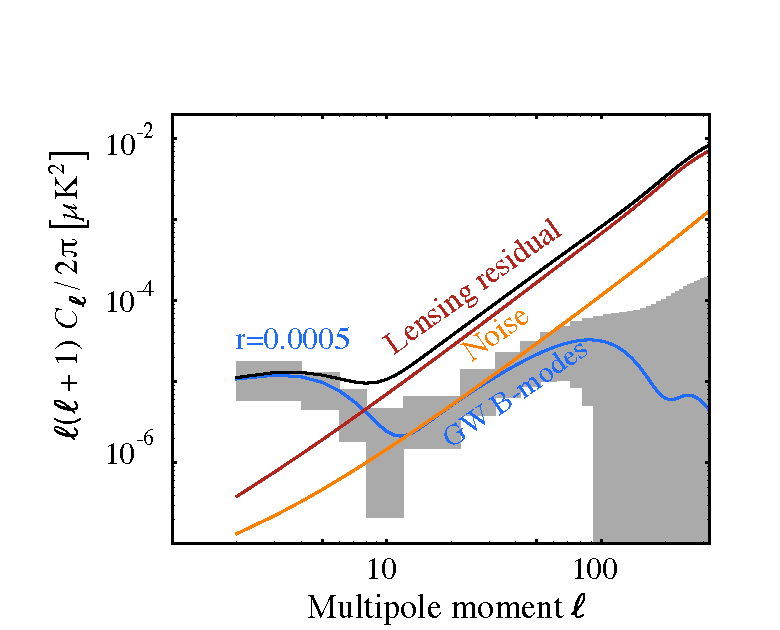
\includegraphics[width=3in]{images/cmbbb_powspec_PICOv4p1_v4.pdf}
\vspace{-0.1in}
\caption{\captiontext With PICO's baseline configuration we will measure the $EE$ (left, red) and lensing $BB$ (green) angular power spectra with high precision (grey). PICO's goal is to detect $r= 5\times 10^{-4}\, (5\sigma)$ (right, grey). This forecast includes PICO's 80\% delensing (red) and foreground separation. The baseline noise level (right, orange) allows detection of even lower levels; we expect foreground separation to limit performance.  As an example we show the total $BB$ spectra on the cleanest $60\%$ of the sky at 75 and 155~GHz (left, purple). The foregrounds largely dominate the cosmological signals. Also shown are measurements of lensing from current experiments (left, orange)~\citep{PB_BB, keisler2015, actpol_lensing_BB, Array:2015xqh}, \planck 's $EE$ measurements (left, dark blue)~\citep{Planck2018_I}, and the $BB$ spectrum produced by an inflationary gravity wave (GW) signal with different values of $r$ (cyan). 
\label{fig:clbb} }
\vspace{-0.05in}
\end{figure}

The strength of the signal, quantified by the tensor-to-scalar ratio $r$, is a direct measure of the expansion rate of the Universe during inflation. Together with the Friedmann equation, it reveals one of the most important characteristics of inflation: its energy scale.\footnote{In some models of inflation the one-to-one correspondence between $r$ and the energy scale of inflation does not hold because there are additional sources of gravitational waves~\cite{Namba:2015gja}. However, in these models the signal is highly non-Gaussian and could be distinguished from models without such sources, for which the signal is Gaussian.}  A detection of $r$  ``would be a watershed discovery'', a quote from the 2010 decadal panel report~\citep{blandford2010}. The combination of data from \planck\ and the BICEP/Keck Array give the strongest constraint to date, $r<0.06\,\, (95\%)$~\citep{bicep_keck2018}. Next decade S3 efforts strive to reach $\sigma(r)=2 \times10^{-3}$~\citep{SOscience, biceparray}.

PICO will detect primordial gravitational waves if inflation occurred at an energy scale of at least $5\times 10^{15}\,\rm{GeV}$, or equivalently $r= 5\times 10^{-4} \, (5\sigma)$ (SO1 in Table~\ref{tab:STM} and Fig.~\ref{fig:clbb}).  A detection will have profound implications for fundamental physics. It will provide evidence for a new energy scale tantalizingly close to the energy scale associated with grand unified theories, probe physics at energies far beyond the reach of terrestrial colliders, and be the first observation of a phenomenon associated with quantum gravity~\cite{Krauss:2013pha}.

%PICO's goal is to detect primordial gravitational waves if inflation occurred at an energy scale of at least $5\times 10^{15}\,\rm{GeV}$, or equivalently $r= 5\times 10^{-4} \, (5\sigma)$ (SO1 in Table~\ref{tab:STM} and Fig.~\ref{fig:clbb}).  A detection will have profound implications for fundamental physics. It will provide evidence for a new energy scale tantalizingly close to the energy scale associated with grand unified theories, probe physics at energies far beyond the reach of terrestrial colliders, and be the first observation of a phenomenon associated with quantum gravity~\cite{Krauss:2013pha}.

There are only two classes of slow-roll inflation in agreement with current data that naturally explain the observed value of the spectral index of primordial fluctuations $n_{\rm s}$~\cite{Aghanim:2018eyx}. The first class is characterized by potentials of the form $V(\phi)\propto\phi^p$. This class includes many of the simplest models of inflation, some of which have already been strongly disfavored by existing observations. Select models in this class are shown as blue lines in Fig.~\ref{fig:nsr}. When the constraints on $n_{\rm s}$ tighten by about a factor of two with the central value unchanged, and the upper limit on $r$ improves by an order of magnitude, this class would be ruled out. 

The second class is characterized by potentials that approach a constant as a function of field value, either like a power law or exponentially. Two representative examples in this class are shown as the green and gray bands in Fig.~\ref{fig:nsr}. This class also includes $R^2$ inflation, which predicts a tensor-to-scalar ratio of $r\sim 0.004$. All models in this class, with a characteristic scale in the potential that is larger than the Planck scale, predict a tensor-to-scalar ratio of $r\gtrsim 0.001$.  PICO will exclude these models with high confidence ($>5\sigma$), and is the only proposed mission for the next decade to reach an exclusion at more than $2\sigma$. While many microphysical models in this second class possess a characteristic scale that is super-Planckian, some have a somewhat smaller scale. One example is the Goncharov-Linde model, which predicts a tensor-to-scalar ratio of $r\sim 4\times 10^{-4}$~\cite{Goncharov:1983mw}, still within $4\sigma$ detection by PICO~(Fig.~\ref{fig:nsr}). There are models with much smaller values that are out of reach.  

%The second class is characterized by potentials that approach a constant as a function of field value, either like a power law or exponentially. Two representative examples in this class are shown as the green and gray bands in Fig.~\ref{fig:nsr}. This class also includes $R^2$ inflation, which predicts a tensor-to-scalar ratio of $r\sim 0.004$. All models in this class, with a characteristic scale in the potential that is larger than the Planck scale, predict a tensor-to-scalar ratio of $r\gtrsim 0.001$. PICO will definitively exclude these models, or will detect gravitational waves; either result will be achieved with more than $5\sigma$ confidence.  While many microphysical models in this second class possess a characteristic scale that is super-Planckian, some have a somewhat smaller scale. One example is the Goncharov-Linde model, which predicts a tensor-to-scalar ratio of $r\sim 4\times 10^{-4}$~\cite{Goncharov:1983mw}, still within $4\sigma$ detection by PICO~(Fig.~\ref{fig:nsr}). There are models with smaller values that are out of reach.  

Distinguishing between models with sub- and super-Planckian characteristic scales would provide much needed guidance to discriminate between classes of ideas for the physics of the earliest moments of our Universe. And this much is clear: PICO will either detect gravitational waves, or, if its required threshold is passed without a detection, most textbook models of inflation will be ruled out and the data would force a significant change in our understanding of the primordial universe.

%Distinguishing between models with sub- and super-Planckian characteristic scales would provide much needed guidance to discriminate between classes of ideas for the physics of the earliest moments of our Universe.

%While many microphysical models in this second class possess a characteristic scale that is super-Planckian, some have a somewhat smaller scale. One example is the Goncharov-Linde model, which predicts a tensor-to-scalar ratio of $r\sim 4\times 10^{-4}$~\cite{Goncharov:1983mw}, still within detection reach by PICO~(Fig.~\ref{fig:nsr}). There are models with significantly smaller values that are out of reach.  

%Distinguishing between models with sub- and super-Planckian characteristic scales would provide much needed guidance to discriminate between classes of ideas for the physics of the earliest moments of our Universe.


\begin{figure}[!thb]
\parbox{4.5in}{\centerline{
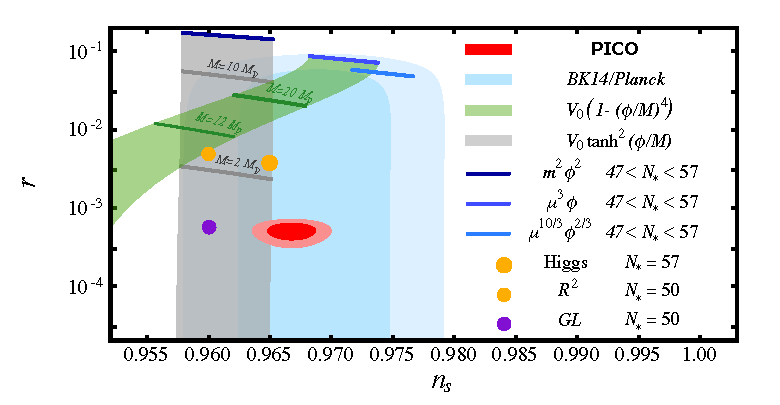
\includegraphics[width=4.5in]{images/nsrlabeledrp0005_PICOv2.pdf} } }
\parbox{1.8in}{
\caption{\captiontext  Current $1\sigma$ and 2$\sigma$ limits on $r$ and $n_{\rm s}$ (cyan) and forecasted constraints for a fiducial model with $r = 0.0005$ for PICO, together with predictions for selected models of inflation. Characteristic super-Planckian scales in the potentials are marked with darker lines. GL is the Goncharev-Linde model (see text). }
\label{fig:nsr}}
\vspace{-0.1in}
\end{figure}

%\paragraph{Observational Considerations}
\noindent$\bullet$ {\bf Observational Considerations} \hspace{0.1in} 
The $BB$ angular power spectrum measured by PICO will have contributions from Galactic sources of emission and `lensing' $B$-modes, created by gravitational lensing of $E$-modes as the CMB photons traverse the gravitational potentials throughout the Universe (Fig.~\ref{fig:clbb} and \S\,\ref{sec:gravitationallensing}). In case of an $r$ detection, there will be two additional features due to the inflationary signal. One is the `recombination peak' at $\ell = 80$ and the other is the `reionization peak' at multipoles of $\ell\lesssim 10$. PICO's strong constraints on $r$ derive from using all available $\ell$ modes.

The Galactic signals act as foregrounds, and uncertainty in the characterization of these foregrounds already limits our ability to constrain $r$. 
%PICO's goal for reaching $\sigma(r) = 1\times10^{-4}$ is driven by estimates of the efficacy of foreground separation, not noise.  
An analytic performance forecast accounting for PICO's statistical noise level and a foreground model that has polarized emission from two components of dust, synchrotron radiation, and correlations between synchrotron and dust emission, gives $\sigma(r) = 2\times10^{-5}$, five times lower than our baseline requirement. This margin allows for degradation in foreground removal through inclusion of physical effects known to exist but not captured in the analytic forecasts. These effects are included in map-based simulations, which indicate that PICO will achieve its requirement; see Section~\ref{sec:signal_separation}. 
%\comor{say more?}

When the tensor-to-scalar ratio $r \simeq 0.01$, the $BB$ lensing and inflation spectra are comparable in magnitude at the recombination peak $(\ell = 80)$. For lower levels of $r$, the lensing $B$-mode dominates, but the $B$-mode maps can be `delensed' if the polarization maps are measured with few-arcmin resolution and sufficient depth~\citep{2004PhRvD..69d3005S,2012JCAP...06..014S}. Forecasts for PICO show that at least 73\% of the lensing $B$-mode power can be removed for the baseline configuration, after accounting for conservative Galactic foreground separation. As much as 85\% will be removed for the CBE and for milder foreground contamination. For measuring the recombination peak, delensing is essential in order to reach PICO's limits on $r$, and this was a driver in choosing the resolution of the instrument. 
% PICO will be relying on its own data to conduct delensing, thus avoiding increased noise from the need to cross-calibrate experiments, identify common observing areas on the sky, not having frequency-band coverage at the appropriate resolution to remove foregrounds, or from other systematic uncertainties.

For the levels of $r$ targeted by PICO, the $BB$ reionization signal $(\ell < 10)$ has a somewhat higher level than the lensing spectrum, but the map-level foregrounds at this angular scale are at least two orders of magnitude brighter.  There are currently no $BB$ measurements at these scales, and no S3 experiments plan to measure $B$-modes that reach to $\sigma(r) < 0.006$ in the lowest multipoles~\citep{class,piper}. PICO's instrument temporal stability, absence of atmospheric noise, full-sky coverage, and unmatched capability to characterize and separate foregrounds make it the most suitable instrument to measure these lowest multipoles (\S\,\ref{sec:signal_separation}).

If an inflationary $B$-mode signal is detected, it is important to characterize its entire $\ell$ dependence in the predicted reionization and  recombination peaks, in order to confirm -- rather than assume -- its expected dependence on angular scale.  Furthermore, the PICO full-sky coverage will enable detection of the recombination peak in several independent patches of the sky, giving an important systematic cross-check. Only a space mission can provide these important benefits. 

\noindent$\bullet$ {\bf Scalar Spectral Index and Non-Gaussianity} \hspace{0.1in} Models of the early Universe differ not only in their predictions for $r$ and the scalar spectral index $n_{\rm s}$, but also for the scale-dependence of $n_{\rm s}$, a parameter commonly called ``the running of $n_{\rm s}$'' and labeled $n_{\rm run}$. PICO will improve $n_{\rm s}$ and $n_{\rm run}$ constraints by a factor of three relative to \planck\ to achieve $\sigma(n_{\rm s})=0.0015$ and $\sigma(n_{\rm run})=0.002$. For many models of inflation, how reheating occurred is unknown, and this translates to different predictions for $n_{\rm s}$ and $n_{\rm run}$~\citep{planck2018_inflation}. PICO's precision is sufficient to distinguish between different possible reheating scenarios at $>3\sigma$ (SO2). 

The simplest models of inflation, in which there is a single inflaton field, predict primordial fluctuations that are very nearly Gaussian with $|f^{\rm local}_{\rm NL}| <1$, where $f^{\rm local}_{\rm NL}$ is a parameter quantifying the level of local non-Gaussianity~\citep{planck2015_17}. A detection of $|f^{\rm local}_{\rm NL}| >1$ points exclusively to models of inflation with multiple fields (Fig.~\ref{fig:fnlconstraint}). 
%, making $\sigma (f^{\rm local}_{\rm NL}) < 1$ a compelling target. 
\planck\ gives a constraint of $f^{\rm local}_{\rm NL} = 0.8 \pm 5 \, (1\sigma)$~\citep{planck2015_17}, and further measurements of the \ac{CMB} alone cannot improve on this constraint by more than a factor of 2--3. However, correlating large-scale structure tracers that have different clustering bias factors can enhance the signature of non-Gaussianity~\citep{2009PhRvL.102b1302S,2018PhRvD..97l3540S,2008PhRvD..77l3514D}. Fig.~\ref{fig:fnlconstraint} shows expected constraints from correlations between the PICO lensing potential maps (\S~\ref{sec:gravitationallensing}) and LSST galaxies. For $f^{\rm local}_{\rm NL}=2$, $3\sigma$ evidence will be reached if large angular scale ($L\ge 8$)\footnote{$L$ refers to multipoles in galaxy clustering fields and in CMB lensing~(\S~\ref{sec:gravitationallensing}), in contrast to the use of $\ell$  for the CMB itself. \label{foot:L}} auto- and cross-correlation spectra can be used. If LSST's auto-correlation can only be used on smaller angular scales $L\ge 20$, the $3\sigma$ evidence weakens to $2\sigma$. 
%Specifically, using data spanning angular scales with $L>6$ a compelling constraint of $|f_{NL}|<1\, (2\sigma)$ will be reached. 

\begin{figure}[h]
\hspace{-0.in}
\parbox{3.0in}{{
% \includegraphics[width=2.95in]{images/PICO_fnl_lmin_PICOv4.1b_deproj0_SENS0.pdf} } }  % pre Dec. 20th version
\includegraphics[width=2.95in]{images/PICO_fnl_lmin_PICOv4.1b_deproj0_SENS0_LSST10yrGoldWithDropouts.pdf} } }   % new version, LSST gold, 10year
\hspace{0.in}
\parbox{3.4in}{
\caption{\captiontext
Cross-correlating PICO's lensing potential map with LSST galaxies will allow detecting or excluding  $f^{\rm local}_{\rm NL}=2$ with $3\sigma$ evidence  if the data can be used at  angular scales $L \ge 8$ (solid black). A detection above $|f^{\rm local}_{\rm NL}| =1$ indicates that inflation is driven by multiple fields; single-field inflation has $|f^{\rm local}_{\rm NL}|<1$ (green region). The \planck\ constraint is $f^{\rm local}_{\rm NL} < 10.8\, (2\sigma)$. The cross-correlations will allow excluding or detecting $f^{\rm local}_{\rm NL}=2\, (2\sigma)$ if LSST data are used only for $L\ge 20$ (dash). Fig.~\ref{fig:sigma8} gives the assumptions used here for the LSST data. 
\label{fig:fnlconstraint}
} }
\vspace{-0.1in}
\end{figure}

%\comor{One can use correlations between large-scale structure tracers with different clustering bias factors and measure the relative difference between their clustering power spectra to effectively cancel cosmic variance~\citep{2009PhRvL.102b1302S,2018PhRvD..97l3540S}; this can constrain physics that affects the biasing of objects on large scales, such as primordial local non-Gaussianity~\citep{2008PhRvD..77l3514D}.  In Fig.~\ref{fig:fnlconstraint} we show the expected constraints for the CMB lensing field as reconstructed with PICO, in cross-correlation with  three years of the LSST survey. It can be seen that depending on the minimal multipole that can be used in the cross correlation, which is uncertain in both LSST and the PICO lensing map, the well-motivated theory target of $\sigma (f_\mathrm{NL}) \simeq 1$ \citep{2014arXiv1412.4671A} can be within reach. Values of $f_\mathrm{NL}$ at or above this level are a generic prediction of multi-field inflationary models.}


\subsubsection{Fundamental Particles: Light Relics, Dark Matter, and Neutrinos}
\label{sec:relics_neutrinos}

%%%%%%%%%%%%%%%%%%%%%%%%%
$\bullet$ {\bf Light Relics} \hspace{0.1in} In the inflationary paradigm, the Universe was reheated to temperatures of 
at least 10 MeV and perhaps as 
high as $10^{12}$ GeV.  At these high temperatures, even very weakly interacting or very massive particles, 
such as those arising in extensions of the Standard Model of particle physics, can be produced in large 
abundances~\cite{1979ARNPS..29..313S,Bolz:2000fu}.  As the Universe expands and cools,
the particles fall out of equilibrium, an event referred to as `decoupling,' and characterized by a decoupling temperature $T_{F}$.  The decoupling leaves observable signatures in the CMB power spectra. Through these effects the CMB is a sensitive probe of neutrino and other particles' properties.  

% sensitive probe of the fundamental particle content in the Universe
% large abundance, but not large enough to leave present day signatures? or they decay?
% don't like the words 'extensions of ...' suggests very unlikely things. 

One particularly compelling target is the effective number of light relic particle species $\Neff$. The canonical value with three neutrino families is $\Neff = 3.046$. Additional light particles contribute a change $\Delta \Neff$ that is a function only of the decoupling temperature and the spin of the particle~$g$. The magnitude of $\Delta\Neff$ is quite restricted, even for widely varying decoupling temperatures $T_{F}$. A range $ 0.027\,g \leq \ \Delta \Neff \leq 0.07\,g$ corresponds to a range in $T_{F}$ spanning decoupling during post-inflation reheating (0.027$g$) down to lower $T_{F}$ with decoupling occurring just prior to the QCD phase transition ($0.07g$).
%Additional light particles contribute a universal change to $\Neff$ that is a function only of the decoupling temperature and the effective degrees of freedom of the particle, $g$. Furthermore, the range of $\Delta\Neff$ is quite restricted, even for widely varying decoupling temperatures $T_{F}$ with the range $ 0.027\,g \leq \ \Delta \Neff \leq 0.07\,g$ corresponding to decoupling at higher temperatures during post-inflation reheating (0.027$g$) to lower temperatures shortly prior to the QCD phase transition ($0.07g$).

Information about $\Neff$ is gleaned primarily from the $TT,\, TE$, and $EE$ power spectra. For an experiment like PICO, which has sufficient resolution to reach a cosmic-variance-limited measurement\footnote{\label{CVL}A measurement is cosmic-variance-limited when the measurement uncertainty is dominated by the statistics of observing the finite number of spherical harmonic decomposition modes available in our Universe.} of $EE$ up to $\ell =2300$, the two additional most important parameters for improving constraints are the fraction of sky observed, $f_{\rm sky}$, and the noise (Fig.~\ref{fig:Neff_future}, left). The PICO baseline will use data from 70\% of the sky to constrain $\Delta \Neff < 0.06 \, (95\%)$ (S04).\footnote{The CMB $EE$ and the Galactic foregrounds $EE$ and $BB$ spectra are comparable in level (Fig.~\ref{fig:clbb}). With 21 frequency bands PICO should be able to separate signals at the mild levels necessary for $EE$ over 70\% of the sky~(\S~\ref{sec:signal_separation}).} This constraint, which is a factor of 4.7 improvement relative to \planck~($\Delta \Neff < 0.28$, 95\%) and will not be matched by any currently funded effort, opens up a new range of temperatures in which to detect the signature of light relic species. If no new species are detected, then the lowest temperature $T_{F}$ at which any %particle with spin 
vector particle (spin 1) could have fallen out of equilibrium will move up by a factor of 400 (Fig.~\ref{fig:Neff_future}, right). 

\begin{figure}[t!]
\begin{center}
\includegraphics[width=0.45\textwidth]{images/Neff_final.pdf}
\includegraphics[width=0.47\textwidth]{images/Tf_pico.pdf}
\vspace{-0.15in}
\caption{ \captiontext PICO will achieve a constraint $\Delta \Neff < 0.06\, (95\%)$ (left, $2\sigma$ contours shown) in the baseline configuration (cross) using its cosmic-variance-limited measurement of $EE$ for $\ell \leq 2300$, and 21 frequency bands to utilize data over 70\% of the sky (5\arcmin\ resolution assumed). This constraint translates to moving up the lowest decoupling temperature $T_{F}$ for particles with spin 1, 1/2, and 0 by factors of 400, 200, and 6, respectively, relative to \planck\ (right, dashed black, only $T_{F}$ for vector particles is shown). We also show the projected vector particle limit for the Simons Observatory~\citep{SOscience}. }
\label{fig:Neff_future}  
\end{center}
\vspace{-0.2in}
\end{figure}

While our theoretical target for $\Neff$ is defined by particles that decoupled long before neutrinos did, there are a number of well-motivated scenarios in which the thermal evolution of the Standard Model is altered after the time of neutrino decoupling.  These scenarios will change the relationship between $\Neff$ as measured in the CMB and the value of $\Neff$ that affects the primordial abundance of the helium fraction $Y_p$ as inferred from big bang nucleosynthesis calculations. 
%While our theoretical target for $\Neff$ is defined by particles that decoupled long before neutrinos did, there are a number of well-motivated scenarios in which the thermal evolution of the Standard Model is altered after the time of neutrino decoupling.  These scenarios will change the relationship between $\Neff$ as measured in the CMB relative to the value of $\Neff$ that affects big bang nucleosynthesis calculations and the production of helium, which is quantified through the helium fraction $Y_p$.  
For example, the decay of a thermal relic into photons after nucleosynthesis would reduce $\Neff$ in the CMB but could leave $Y_p$ unaltered from its Standard Model value.  PICO will make a simultaneous measurement of $\Neff$ and $Y_p$ with $\sigma(\Neff) = 0.08$ and $\sigma(Y_p) =0.005$, giving a 2\% uncertainty on the value of $Y_p$. These uncertainties are equivalent to those available with other astrophysical measurements, but the systematic uncertainties are entirely different. Systematic uncertainties currently limit our knowledge of $Y_{p}$. 

%%%%%

\noindent$\bullet$ {\bf Dark Matter} \hspace{0.1in} Cosmological measurements have already confirmed the existence of one relic that lies beyond the Standard Model: dark matter. \ac{CMB} experiments are effective in constraining dark matter candidates in the lower mass range, which is not available for terrestrial direct detection experiments~\citep{Slatyer2009,Galli2009,Huetsi2009,Huetsi2011,Madhavacheril:2013cna,Green:2018pmd}. 

Interactions between dark matter and protons in the early Universe create a drag force between the two cosmological fluids, damping acoustic oscillations and suppressing power in density perturbations on small scales. As a result, the CMB temperature, polarization, and lensing power spectra are suppressed at high multipoles relative to a Universe without such drag forces.  This effect has been used to search for evidence of dark-matter--proton scattering over a range of masses, couplings, and interaction models~\citep{2002astro.ph..2496C, 2004PhRvD..70h3501S, Dvorkin:2013cea, 2018PhRvL.121h1301G,2018arXiv180108609B, 2018PhRvD..97j3530X, 2018arXiv180800001B, 2018PhRvD..98b3013S}, to test the possibility of an interacting dark-matter sub-component~\citep{2018arXiv180800001B}, and to provide consistency tests of dark matter in the context of the anomalous 21-cm signal reported by the EDGES collaboration~\citep{2018Natur.555...71B,2018Natur.555...67B,2018arXiv180800001B,2018arXiv180711482K}.
 
PICO's constraining power comes primarily from making high \ac{SNR} maps of the lensing-induced deflections of polarized photons, which are discussed in Section~\ref{sec:extragalacticsci}.  For a spin-independent velocity-independent contact-interaction, chosen as our fiducial model, PICO will improve upon \planck 's dark matter cross-section constraints by a factor of 25 over a broad range of candidate masses that are largely unavailable for traditional direct detection experiments (Fig.~\ref{fig:DM_baryons}, right). 
%The constraints are complementary to those forthcoming from direct detection experiments, which are more sensitive at the high mass range.  
%\comor{need to decide what to do with this section.}
%which is largely unavailable to traditional direct detection experiments

\begin{figure}[t]
\begin{center}
\includegraphics[width=0.50\textwidth]{images/pico_dd4.pdf}
\includegraphics[width=0.48\textwidth]{images/Mnu_tauprior_final.pdf}
\vspace{-0.15in}
\caption{\captiontext {\bf Left:} PICO will give a factor of 25 more stringent constraint on the spin-independent velocity-independent dark matter scattering cross-section (dashed) relative to current \planck\ 95\% confidence limit (red)~\citep{2018PhRvL.121h1301G}. Terrestrial direct detection experiments are expected to give complementary and stronger constraints, but only for the higher dark matter masses (grey)~\cite{2018PhRvD..97l3013K}. 
{\bf Right:} Using a cosmic-variance-limited (CVL) measurement of $\tau,\, \sigma(\tau)=0.002$, \ac{BAO} information from DESI, and separation of foregrounds over 70\% of the sky, PICO will reach $\sigma(\Sigma m_{\nu}) = 14$~meV (contours), giving at least a $4\sigma$ detection of the minimal expected sum of neutrino masses $\Sigma m_{\nu} = 58$~meV. 
\label{fig:DM_baryons} }
\end{center}
\vspace{-0.2in}
\end{figure}
%

The axion is another dark matter candidate that is well motivated by string theory~\citep{Arvanitaki_etal} and that is consistent with straightforward extensions of the Standard Model of particle physics~\citep{peccei,weinberg,wilczek}. For an axion mass in the intermediate range $10^{-30} < m_a< 10^{-26} $~eV, current measurements constrain its fraction to be $\le 2$\% $(1\sigma)$ of the total dark-matter density. If 2\% of the total dark content is made of axions, PICO's measurement of the $TT$, $TE$ and $EE$ spectra with additional constraints from the lensing reconstruction will detect this species at between $7$ and $13\sigma$, depending on the mass range. %, as shown in Figure~\ref{fig:axions}. 
This is an average improvement of a factor of 10 relative to \planck .
% and a factor of two relative to the combination of \planck\ and S3, respectively, profoundly shaping our understanding of the nature of dark matter and its small-scale clustering. 

\noindent$\bullet$ {\bf Neutrino Mass} \hspace{0.1in} \label{neutrino_fundamental} The origin and structure of the neutrino masses is one of the great outstanding  questions about the nature of the Standard Model particles.  
%Measurements of neutrinos in the lab have revealed much  about the mass differences and mixing angles.  
Cosmology offers a  measurement of the sum of the neutrino masses $\sum m_\nu$ through the gravitational influence of the non-relativistic  cosmic neutrinos.  The current measurement of $\Neff = 2.99 \pm 0.17$~\citep{Planck2018_VI} already confirms the existence of these neutrinos at $>10\sigma$ and their mass implies that they will contribute to the matter density at low redshifts.  The best current mass constraint arises from a combination of  \planck~and BOSS \ac{BAO} giving $\sum m_\nu < 0.12$ eV (95\%) \cite{Planck2018_VI}.

Cosmological measurements are primarily sensitive to the suppression of power on small scales after the neutrinos become non-relativistic, which can be measured via CMB lensing (\S~\ref{sec:gravitationallensing}), or weak lensing in galaxy surveys.  However, these measurements are limited by our knowledge of the amplitude of the primordial fluctuation power spectrum $A_s$ because they only constrain the combination $A_s e^{-2 \tau}$, where $\tau$ is the optical depth to reionization. Although many astrophysical surveys hope to detect $\sum m_\nu$, any detection of the minimum value expected from particle physics, $\sum m_\nu = 58$~meV, at more than $2 \sigma$, will require a better measurement of $\tau$.
% and thus do not provide a high-precision measurement of either $A_s$ or $\tau$ separately.  \comor{we mention 'galaxy survey', but don't complete the thread of thought. Do we mean to say that the galaxy survey will be limited by the same degeneracy?}

The strongest constraints on $\tau$ come from the $EE$ spectrum at $\ell < 10$, which requires measurements over the largest angular scales  and good separation of Galactic foreground sources of emission. The best current measurement with $\sigma({\tau}) = 0.007$ is from \planck~\cite{Planck2018_VI}. With this uncertainty in $\tau$ one is limited to  $\sigma(\sum m_\nu) \gtrsim 25$ meV, after including forthcoming \ac{BAO} information (Fig.~\ref{fig:DM_baryons}, right); no other survey or cosmological probe will improve this constraint, unless a more accurate measurement of $\tau$ is made. One of the S3 experiments is attempting to measure the lowest $\ell$s and improve upon the \planck\ precision by a factor of about two~\citep{class}. A space mission with its access to the entire sky and broad frequency coverage is the most suitable platform for the measurement~(\S~\ref{sec:signal_separation} and \S~\ref{sec:complementarity}). PICO will reach the cosmic-variance limit uncertainty on $\tau$, $\sigma(\tau) = 0.002$~(\S~\ref{sec:luminoussources}), and using its deep CMB lensing map (\S~\ref{sec:gravitationallensing}) will therefore reach $\sigma(\sum m_\nu) = 14$ meV when combined with measurements of \ac{BAO} from DESI or Euclid~\cite{Levi:2013gra}.
%(without \ac{BAO} data the constraint is $\sigma(\sum m_\nu) = 43$ meV).
This measurement will give a $4\sigma$ detection of the minimum sum (SO3). 

%Robustly detecting neutrino mass at  $> 3\sigma$ in any cosmological setting is only possible with an improved measurement of $\tau$, like the one achievable with PICO. This measurement will give $\sum m_\nu>0$ at greater than $4\sigma$ or would exclude the inverted hierarchy ($\sum m_\nu > 100$ meV) at 95\% confidence, depending on the central value of the measurement.  Lab-based measurement could determine the hierarchy before PICO, but only cosmology can measure $\sum m_\nu$.

%%%%%%%%%%%%%%%%%%%%%%%%%

\subsubsection{Fundamental Fields: Primordial Magnetic Fields and Cosmic Birefringence}

$\bullet$ {\bf Primordial Magnetic Fields} \hspace{0.1in} One of the long-standing puzzles in astrophysics is the origin of observed 1--10~$\mu$G galactic magnetic fields~\citep{Widrow:2002ud}. Producing such fields through a dynamo mechanism requires a primordial seed field~\citep{Widrow:2011hs}. Moreover, $\mu$G-strength fields have been observed in proto-galaxies that are too young to have gone through the number of revolutions necessary for the dynamo to work~\citep{Athreya:1998}. A primordial magnetic field (PMF), present at the time of galaxy formation, could provide the seed or even eliminate the need for the dynamo altogether. Specifically, a 0.1~nG field in the intergalactic plasma would be adiabatically compressed in the collapse to form a $\sim$1~$\mu$G galactic field~\citep{Grasso:2000wj}.
PMFs could have been generated in the aftermath of phase transitions in the early Universe~\citep{Vachaspati:1991nm}, during inflation~\cite{Turner:1987bw,Ratra:1991bn}, or at the end of inflation~\cite{DiazGil:2007dy}. A detection of PMFs with the CMB would be a major discovery because it would establish the magnetic field's primordial origin, signal new physics beyond standard models of particle physics and cosmology, and discriminate among different theories of the early Universe~\cite{Barnaby:2012tk,Long:2013tha,Durrer:2013pga}.

The current CMB bounds on PMF strength are $B_{\rm 1\,Mpc}<1.2$ nG at 95\% CL for the scale-invariant~PMF spectrum \cite{Planck2015PMF,Kunze2015,Chluba2015PMF,Zucca:2016iur}, based on measurements of the $TT$, $TE$, $EE$, and $BB$ spectra.\footnote{It is conventional to quote limits on the PMF strength smoothed over a $1$~Mpc region in comoving units,  i.e., rescaled to $z=0$: $\mathbf{B}_{\rm today} = a^2\mathbf{B}(a)$.} 
%In particular, PMF sourced vector modes contribute to the $BB$ power spectrum at high $\ell$ \cite{Lewis:2004ef}. 
The much more accurate measurement of $BB$ by PICO would only marginally improve the PMF bound because CMB spectra scale as $B^4_{\rm 1\,Mpc}$. However, Faraday rotation provides a signature that scales linearly with the strength of PMFs~\cite{Kosowsky:1996yc}. It converts CMB $E$ modes into $B$ modes, generating mode-coupling $EB$ and $TB$ correlations. So far this signature has been out of reach because prior experiments did not have sufficient sensitivity. Using Faraday rotation, PICO will probe PMFs as weak as 0.1~nG ($1\sigma$), a precision that already includes the effects of imperfect lensing subtraction, Galactic foregrounds~\cite{Oppermann:2011td,De:2013dra,Pogosian:2013dya}, and other systematic effects. With this precision, which is a factor of five stronger than achievable with S3 experiments, PICO can conclusively rule out the purely primordial (i.e., no-dynamo driven) origin of the largest galactic magnetic fields. \\
%
$\bullet$ {\bf Cosmic Birefringence} \hspace{0.1in}
A number of well-motivated extensions of the Standard Model involve (nearly) massless axion-like pseudo-scalar fields coupled to photons via the Chern-Simons interaction term~\citep{Freese:1990rb,Frieman:1995pm,Carroll:1998zi,Kaloper:2005aj}. These couplings also generically arise within quintessence models for dark energy~\citep{Carroll:1998zi}, chiral-gravity models~\citep{2008PhRvL.101n1101C}, and models that produce parity-violation during inflation~\cite{Gluscevic:2010vv}. Regardless of the source of the parity-violating coupling, its presence may cause cosmic birefringence -- a rotation of the polarization of an electromagnetic wave as it propagates across cosmological distances~\cite{Harari:1992ea,Carroll:1989vb,Carroll:1998zi}. Cosmic birefringence converts primordial $E$-modes into $B$-modes, producing $TB$ and $EB$ cross-correlations whose magnitude depends on the statistical properties of the rotation field in the sky~\cite{Kamionkowski:2008fp,Gluscevic:2009mm,Gluscevic:2012me}. Previous studies have constrained both a uniform rotation angle as well as anisotropic rotation described by a power spectrum \cite{Gluscevic:2012me}. The current bound on a uniform angle is 30\arcmin\ (68\%)~\cite{Planck2016_XLIX}, and the bound on the amplitude of a scale-invariant rotation angle spectrum, which could be caused by fluctuations in a light pseudo-scalar field present during inflation~\cite{Pospelov:2008gg}, is 0.11~deg$^2$ (95\%)~\citep{Array:2017rlf}). Using the combination of five bands in the 70--156~GHz range, PICO will reduce the 95\% CL bound on the uniform rotation angle by a factor of 300, to 0.1\arcmin.  
%, assuming that the beam can be calibrated to reach the main science goals without \emph{assuming} vanishing parity-odd spectra of $EB$ and $TB$ type. 
The 95\% CL bound on the amplitude of a scale-invariant rotation spectrum will be reduced by a factor of 275 to $4\times10^{-4}$~deg$^2$, giving important constraints on string-theory-motivated axions~\cite{Svrcek:2006yi,Pospelov:2008gg}.


%The simplest model for late-time acceleration of the Universe is with a slowly-evolving scalar field, also called quintessence~\cite{Carroll:1998zi}. Such a field generically couples to electromagnetism through a Chern Simons-like term, and causes linear polarization of photons propagating cosmological distances to rotate. This is known as cosmic birefringence~\cite{Carroll:1998zi}. The birefringence converts primordial $E$-modes into $B$-modes. It thus produces parity-violating $TB$ and $EB$ cross-correlations whose magnitude depends on the statistical properties of the rotation field in the sky~\cite{Kamionkowski:2008fp,Gluscevic:2009mm}. There are no theoretical predictions for the level of birefringence, but if observed, it would be evidence for physics beyond the standard model and a potential probe of dark-energy microphysics~\citep{Gluscevic:2009mm,Caldwell:2011,yadav2009}. 


\end{document}



\subsection{Extragalactic Science}
\documentclass[PICOReport.tex]{subfiles}

\begin{document}

%To cover: Galaxy Formation, Clusters, Reionization, point sources (probably moves to a new section called 'Legacy Science')

{\bf The Formation of the First Luminous Sources}\\
The reionization of the Universe, which according to current measurements takes place near a cosmic age of $\sim$700 million 
years~\citep{planckreion}, imprints multiple signals in the temperature and polarization of the CMB.  In polarization, the most 
important signal is an enhancement of power in the E-mode spectrum at large angular scales $\ell \simlt 20$. 
%scale $E$-mode power sourced by the scattering of the temperature quadrupole during this epoch.  
This signal gives a direct measurement of the optical depth to the reionization epoch $\tau$, and thus to the 
mean redshift of reionization $Z_{re}$, with very little degeneracy with other cosmological parameters; see Figure~\ref{fig:ReionizationPICO}. 
%In contrast, inference of $\tau$ from the $TT$ power spectrum is hindered by its direct degeneracy with the scalar fluctuation amplitude.  
The mean redshift of reionization $Z_{re}$ (when $50$\% of the cosmic volume was reionized) depends sensitively 
on the nature of the ionizing sources.  For example, it is currently unknown whether star-forming galaxies or more exotic 
sources such as supermassive black holes drove the reionization process.  \comor{is this THE question, or are there other 
examples? Would the answer change $Z_{re}$?}
%The PICO constraint on $\tau$ is converted to a constraint on $z_{re}$ in Fig.~\ref{fig:ReionizationPICO}, which is further discussed below.
Furthermore, the detailed shape of the low-$\ell$ $E$-mode power spectrum is sensitive to the reionization history 
itself (i.e., $d\tau/dz$), and will provide information beyond that captured in $\tau$ alone.  For example, it has been 
argued that \planck data show evidence for an extended tail of reionization out to $z \approx 15$-$20$~\cite{Miranda2017}.  
A cosmic-variance-limited measurement of the large-scale $E$ modes, as obtained by PICO, will settle this question.  
%The measurement of $\tau$ constrains the mean redshift of reionization, $z_{re}$ (i.e., when $50$\% of the cosmic volume was reionized), which depends sensitively on the nature of the ionizing sources.  For example, it is currently unknown whether star-forming galaxies or more exotic sources (e.g., supermassive black holes) drove the reionization process.  The PICO constraint on $\tau$ is converted to a constraint on $z_{re}$ in Fig.~\ref{fig:ReionizationPICO}, which is further discussed below.  %\comor{not sure about the comment in the parenthesis. $\tau$ is in the STM to 'distinguish between models that describe the formation of the earliest stars' , but that aspect is not highlighted here ...(??). the paragraph also doesn't reference Figure 3, should it?} 
 
Large-scale $EE$ power spectrum measurements are a unique and crucial observable for many aspects of cosmology \comor{which many}.  
If measurements of $\tau$ are not improved beyond the current uncertainties from {\em Planck}, inference of several new signals 
of cosmological physics (e.g., neutrino mass) will be severely hindered \comor{which other new signals}.  
PICO is the ideal experiment to make this measurement.  
Its noise level and frequency coverage permit a cosmic-variance-limited constraint on $\tau$, i.e., $\sigma(\tau) \approx 0.002$, which we have verified with explicit forecasts including foregrounds. 
% We verify this expectation via an explicit forecast following the methodology described in~\citet{errard_feeney_2015}, assuming PICO measurements of the $TT$, $TE$, $EE$, $BB$, and $\phi\phi$ power spectra, with the latter inferred via the iterative $EB$ estimator.  The polarized dust and synchrotron levels match those measured by {\em Planck}~\citep{PlanckFG2015}, including spatial variations, and are cleaned using a parametric maximum-likelihood approach.  Fitting a $\Lambda$CDM$+r$ model, for both the PICO ``requirements'' and ``CBE'' configurations, we find $\sigma(\tau) = 0.002$.  With the exquisite control of systematics needed for the much smaller primordial $BB$ signal, these are not a concern for $EE$ (and hence $\tau$).

In temperature, the most important imprint of reionization is that sourced at small angular scales by the ``patchy'' kinematic 
Sunyaev-Zel'dovich (kSZ) effect, due to the peculiar velocities of free electron bubbles around ionizing sources (e.g., galaxies or quasars).  
The total kSZ power spectrum receives contributions from both the patchy reionization signal and ``late-time'' sources, e.g., the intergalactic and 
intracluster media.  The reionization and late-time signals are expected to have comparable 
amplitudes~\citep{Shaw2012,MMS2012,Battaglia2013}.  With constraints on the late-time contribution from other 
information (e.g., cross-correlations), effective small-scale foreground removal, and with the primary CMB $TT$ power 
spectrum constrained by inference from the $EE$ power spectrum, it is possible to extract reionization constraints from the 
small-scale kSZ power spectrum~\citep{calabrese/etal/2014}.  The most directly constrained quantity is the duration of 
reionization, $\Delta z_{re}$. \comor{if pico is not providing kSZ constraints, only S3 does, there 
is no need to dwell on it at all, I think.  Nick, can you condense this?}

Fig.~\ref{fig:ReionizationPICO} presents forecasts for reionization constraints in the $z_{re}$-$\Delta z_{re}$ parameter space obtained 
from PICO's measurement of $\tau$ in combination with ground-based Stage-III (CMB-S3) constraints on the kSZ power spectrum.  
Constraints from existing Planck data and observations at other wavelengths are also presented.  The PICO measurement of $\tau$ 
is essential for breaking degeneracies \comor{does not appear to be borne out by the figure} and allowing simultaneous, 
precise constraints to be placed on both the mean redshift and 
duration of reionization.  Fig.~\ref{fig:ReionizationPICO} also shows curves of constant source efficiency (i.e., the efficiency of 
ionizing photon production) and constant intergalactic medium opacity (i.e., the photon mean free path).  PICO will allow 
simultaneous constraints to be placed on these physical parameters, yielding important information on the nature of the 
first luminous sources (e.g., star-forming galaxies or quasars predict significantly different values for these parameters).

\begin{figure}
\hspace{-0.in}
\parbox{3.1in}{\centerline {
\includegraphics[width=3.0in]{images/Reionization_Contours_zbar_delz_PICO_NEW.pdf} } }
\hspace{0.in}
\parbox{3.5in}{
\caption{\label{fig:ReionizationPICO} Summary of constraints on the mean redshift and duration of reionization. The forecasts show 68\% and 95\% confidence-level contours for PICO combined with CMB-S3 experiments and Planck combined with CMB-S3 experiments (dark blue and dashed blue, respectively). The solid black lines illustrate how the IGM opacity and source efficiency model parameters map onto this parameter space. The forecasted PICO constraints are compared to: current exclusion limits for the mean redshift of reionization from Planck, shown by the yellow bands \citealp{planck2018:parameters}; recent exclusion limits from the global 21 cm signal measured by EDGES, shown with the red band \citealp{edges2017}; exclusion limits from measurements of the Gunn-Peterson trough from fully absorbed Lyman$\alpha$ in quasar spectra, shown by the grey band \citealp{Fan2006}; exclusion limit on the duration of reionization from Planck and SPT data, shown by the green band \citealp{planck_reio:2016}.} }
\vspace{-0.1in}
\end{figure}

In addition to these signals, reionization also leaves specific non-Gaussian signatures in the CMB.  In particular, patchy reionization 
induces non-trivial 4-point functions in both temperature~\citep{SmithFerraro2017} and polarization~\citep{DvorkinSmith2008}.  The 
temperature 4-point function can be used to separate reionization and late-time kSZ contributions.  Combinations of temperature and 
polarization data can be used to build quadratic estimators for reconstruction of the patchy $\tau$ field, analogous to CMB lensing 
reconstruction.  These estimators generally require high angular resolution, but also rely on foreground-cleaned CMB maps.  Thus, 
while PICO alone may not enable high S/N reconstructions, its high-frequency channels --- which have better than 2 arcmin 
resolution and observe at frequencies that have yet to be demonstrated from the ground --- will enable these estimators to be 
robustly applied to ground-based CMB data sets, a strong example of ground-space complementarity.
\comor{if pico is complementarity by {\it only} providing foreground maps at sufficiently high resolution, I think we should move 
this to the 'complementarity'. It is not a direct science goal or outcome.}

% JCH: I checked the Smith-Ferraro 4-pt estimator, and PICO does not have sufficient resolution to do this (see Fig. 3 of https://arxiv.org/pdf/1803.07036.pdf )

\comor{The Sections below need to be rearranged to match other Science Objective(s) from the STM, but to also relay the breadth of science reachable by PICO, even if those goals are not in the STM.}

{\bf Structure Formation via Gravitational Lensing}

Matter between us and the CMB last-scattering surface deflects the path of photons through gravitational lensing, encoding the 3-dimensional 
matter distribution across the entire visible universe onto a 2-dimensional image. The specific quantity being mapped is the projected gravitational 
potential $\phi$ that is lensing the CMB, commonly called the `lensing map', from which we form an angular power spectrum $C_{\ell}^{\phi \phi}$.  
Both the temperature and polarization maps of the CMB are affected by lensing, and subsequently the angular power spectra. One of the most 
pronounced effects is the existence of the `B-mode lensing power spectrum'; see Figure~\ref{??}.^\footnote{It is a result of graviational lensing of E-modes into B-modes.}  
While \planck  had a signal-to-noise ratio (SNR) of 40~\cite{ } \comor{map or phi-phi?}, 
the PICO combination of resolution, sensitivity and sky coverage \comor{is sky coverage important} enables a measurement with SNR of 638 and 737 
for the required and CBE configurations, respectively. When accounting for possible foreground contamination, its broad frequency coverage leads 
to a reduction of SNR of less than 20\%; see Figure~\ref{fig:lensingNoisePICO}.  
% say something about "the best measurement"...?
The value of such a deep lensing map is immense, as has already been seen with {\it Planck}. The lensing map is most sensitive to 
structures at redshift $z \simeq 2$ and down to scales of approximately ten arcminutes \comor{talk to Alex; there is a
comment about `wide range of angular scales'}.  
Tomographic cross-correlations of the lensing map with samples of galaxies and quasars will yield constraints 
on structure formation out to redshifts inaccessible to galaxy surveys or galaxy weak lensing maps on their own.
%, particularly through the high-S/N cross-correlation science that will be enabled.  
 These measurements will yield constraints on dark energy, modified gravity, and neutrino mass. Note that this neutrino mass constraint is 
 complementary to that inferred from the CMB lensing auto-power spectrum described earlier \comor{check how we referred to it
 earlier. do we have quantitative values for the constraints?}.  The measurements will constrain the properties of quasars and 
 other high-redshift astrophysics, e.g., a precise determination of the quasar bias (and hence host halo mass) as a function of their 
 properties, such as (non-)obscuration \comor{need to talk to Alex/Marcel about this}.  We provide further quantitative cross-correlation forecasts below.  

% Fig.~\ref{fig:lensingNoisePICO} shows per-mode noise curves for the reconstruction of CMB lensing from PICO, demonstrating the wide range of angular scales over which the matter density field will be  mapped.  \textbf{Add brief discussion of foreground robustness demonstrated in Fig.~\ref{fig:lensingNoisePICO}}

\begin{figure}
\hspace{-0.in}
\parbox{3.1in}{\centerline {
\includegraphics[width=3.0in]{images/lensingNoisePICO.pdf} } }
\hspace{0.in}
\parbox{3.5in}{
\caption{\label{fig:lensingNoisePICO} Lensing noise curves for various experimental configurations, showing the noise per mode of the reconstructed lensing field.  The signal curve, i.e., the CMB lensing power spectrum, is shown in grey; mapping of the matter density field is possible on scales where the noise curves fall below this signal.  Solid curves are for the ``required'' noise level while dashed curves are for the ``CBE'' noise level.  In blue are shown noise curves without cleaning foregrounds, while in brown are the results when performing this cleaning, which adds robustness at the cost of statistical power.%% Shown in solid are the performance of the $EB$ polarization estimator, including iterated delensing; this estimator performs best on large angular scales.  On smaller angular scales the temperature ($TT$) estimator shows the best performance. The associated signal to noise ratio for the lensing power spectrum is 570 for the 'requirement' configuration and 650 for the 'CBE' configuration. \textbf{Update with foreground-cleaned polarization noise curve(s) to demonstrate robustness.} }
}
\vspace{-0.1in}
\end{figure}


%Measurements of the CMB reveal structure imprinted not only at the early time of recombination, but also at nearly every significant ensuing epoch in cosmic history.  In particular the matter between us and the CMB last-scattering surface will deflect the path of CMB photons, a process known as gravitational lensing.  Although the lensing of the CMB is a weak signal, targeted statistical estimators enable its extraction.  Measurements of the lensing signal have rapidly progressed, from the first detections in 2007-8 \citep{2007PhRvD..76d3510S, 2008PhRvD..78d3520H} to the recent $40\sigma$ measurement by the {\it Planck} team \cite{2018arXiv180706210P}.  When applied to a rich dataset such as that expected from the PICO satellite, these estimators will provide a map of all the matter in the Universe in projection, with the most sensitivity at redshift $z \simeq 2$ and down to scales of approximately ten arcminutes.  

%Forecasts show that the power spectrum of lensing in the PICO CMB map can be detected at approximately 580$\sigma$ or 650$\sigma$ for the requirement or CBE configurations, respectively.  Such high-S/N measurements are more than an order of magnitude improvement over the current state of the art, obtained by the {\it Planck} team.  The legacy value of the PICO CMB lensing map is immense, as has already been seen with {\it Planck}, particularly through the high-S/N cross-correlation science that will be enabled.  For example, tomographic cross-correlations of the PICO CMB lensing map with samples of galaxies and quasars will yield constraints on structure formation out to redshifts inaccessible to galaxy surveys or galaxy weak lensing maps on their own.  These measurements will yield constraints on dark energy, modified gravity, and neutrino mass (complementary to the neutrino mass inferred from the CMB lensing auto-power spectrum described earlier).  In addition, PICO CMB lensing cross-correlations will yield constraints on the properties of quasars and other high-redshift astrophysics, e.g., a precise determination of the quasar bias (and hence host halo mass) as a function of their properties, such as (non-)obscuration.  We provide further quantitative cross-correlation forecasts below.  Fig.~\ref{fig:lensingNoisePICO} shows per-mode noise curves for the reconstruction of CMB lensing from PICO, demonstrating the wide range of angular scales over which the matter density field will be mapped.  \textbf{Add brief discussion of foreground robustness demonstrated in Fig.~\ref{fig:lensingNoisePICO}}

{\bf Gravitational Lensing as Noise for Gravity Wave Science}

\comor{\SH version, need to reconcile with the paragraph below. } 
When the tensor to scalar ratio $r \simeq 0.01$, the B-mode lensing power spectrum and the one from gravity waves have approximately 
the same level at $\ell = 80$. For lower levels of $r$, the stronger gravity wave peak is masked by E-mode photons that are lensed into B. 
But the B-mode maps can be `delensed'~\cite{??}. The effect of lensing on E and B maps can be determined and undone if these maps are 
measured with few arcmin resolution and with sufficient depth. Forecasts show that at a minimum 73\% of lens-induced $B$ mode power will 
be removed for the PICO 'requirement' configuration, after accounting for foreground subtraction. 80\% will be removed if the foregrounds 
do not degrade the inherent SNR, rising to 85\% for the CBE. Without delensing PICO determination of $r$ would be limited to $r>??$. 
We emphasize that PICO will be relying on its own data to conduct the delensing and foreground cleaning, thus avoiding reduced efficacy arising 
from the need to cross-calibrate experiments, identify common observing areas on the sky, or not having frequency band coverage at the appropriate resolution to remove foregrounds. 


\comor{AVE version}
Lensing breaks the highly symmetric configuration of primordial density fluctuations appearing as $E$ modes on the sky, turning some of these into $B$ modes.  If not accounted for, this effect yields a noise floor on the large-scale $B$ modes that can be measured from the early Universe.  However, maps of $E$ modes and of the lensing field, both of which will be obtained with PICO data, can be used together to create a template for these lensed $B$ modes.  This template can then be subtracted from the measured $B$ modes to obtain improved performance, in a process known as ``delensing'' \citep{2004PhRvD..69d3005S,2012JCAP...06..014S}.  Forecasts show that up to 80\% of the lens-induced $B$ mode power can be removed in the 'requirement' configuration, with this number becoming 85\% for the current best estimate.  

\textbf{To be added:}

\textbf{- CMB halo lensing forecast (Jim, Jean-Baptiste)}

\textbf{- Cross-correlation forecast (Marcel)}


{\bf Physics of Galaxy Formation via the Sunyaev-Zel'dovich (SZ) Effects}

Not all CMB photons propagate through the universe freely; about 6\% are Thomson-scattered by free electrons in the intergalactic medium (IGM) and intracluster medium (ICM). These scattering events leave a measurable imprint on CMB temperature fluctuations, and they contain a wealth of information from how structure grows to the thermodynamic history of baryons. A fraction of these photons are responsible for the Sunyaev--Zel'dovich effects~\citep{SZ1969,SZ1972}. The thermal SZ effect (tSZ) is the increase in energy of CMB photons due to scattering off hot electrons. This results in a spectral distortion
%, proportinal to the electron pressure,
 of the CMB blackbody that corresponds to a decrement in CMB temperature at frequencies below 217 GHz and an increment at frequencies above. The kSZ effect is the Doppler shift of CMB photons Thomson-scattering off free electrons that have a non-zero peculiar velocity with respect to the CMB rest frame. 
%This produces small shifts in the CMB temperature proportional to the radial velocity of the object and its optical depth.
The amplitudes of the tSZ and kSZ signals are proportional to the integrated electron pressure (tSZ) and momentum (kSZ) along the line of sight, respectively.  They thus contain information about the thermodynamic properties of the IGM and ICM.
%since their magnitudes are proportional to the integrated electron pressure (tSZ) and momentum (kSZ) along the line of sight.
The tSZ effect can be used to measure ensemble statistics of galaxy clusters, which contain cosmological information, as well as to provide uniform cluster samples for galaxy formation studies in dense enviroments.
%
%\item Cosmological parameters from the abundance of tSZ-detected clusters and statistics of component-separated tSZ maps.
%\item Thermodynamic properties of galaxies, groups, and clusters from combined tSZ and kSZ cross-correlation measurements.
%\item Measurements of peculiar velocities, which are powerful cosmological probes on large scales, through the kSZ effect.
%\item Patchy reionization which imprints the CMB through higher order moments of the kSZ effect.

{\bf Galaxy Clusters}

%Through the tSZ PICO will produce a large all sky catalog of 

Galaxy clusters found via the tSZ  effect provide a well-defined sample with a simple-to-model selection function. Sample of clusters such as these are easy to use for cosmological inferences and studies of galaxy evolution in dense environments. 
Points to still hit.
High z sample,
Numbers -- Nick and Jim should cross-check,
most massive cluster all over the whole sky,
Cosmology.

{\bf Compton-$y$ map and tSZ auto-power spectrum}

In addition to finding individual clusters, multifrequency CMB data also allow the reconstruction of full-sky maps of the thermal SZ signal (Compton-$y$ maps) via foreground removal algorithms similar to those used to obtain cleaned maps of the CMB.  With its extremely low noise and broad frequency coverage, PICO will yield a definitive Compton-$y$ map over the full sky, with high S/N down to angular scales of a few arcminutes.  We quantify this expectation by reconstructing the Compton-$y$ field using the needlet internal linear combination (NILC) algorithm~\cite{Delabrouille2009} applied to sky simulations generated with the \planck sky model, with maps at all PICO frequencies (with appropriate noise added).  The error bars on the reconstructed tSZ power spectrum are shown in Fig.~\ref{fig:PICO_tSZ_PS}, in comparison to current measurements.  The total $S/N = 1270$ for the PICO CBE configuration, with the PICO requirements configuration only $\approx 10$\% lower.  This is nearly two orders of magntiude larger than the current S/N from \planck.

Extremely strong constraints on models of astrophysical feedback will be obtained from the analysis of the PICO $y$-map, both from its auto-poewr spectrum and from cross-correlations with galaxy, group, cluster, and quasar samples.  Like the CMB lensing map described above, the legacy value of the PICO $y$-map will be immense.  As an example, we forecast the detection of cross-correlations between the PICO $y$-map and galaxy weak lensing maps constructed from LSST and WFIRST data.  Considering the LSST ``gold'' sample with a source density of 26 galaxies/arcmin${}^2$ covering 40\% of the sky, we forecast a detection of the tSZ -- weak lensing cross-correlation with S/N = 3000.  At this immense significance, the signal can be broken down into dozens of tomographic redshift bins, yielding a precise breakdown of the evolution of thermal pressure over cosmic time.  For PICO and WFIRST (assuming 45 galaxies/arcmin${}^2$ covering 5.3\% of the sky), we forecast S/N = 1100 for the tSZ -- weak lensing cross-correlation.  The WFIRST galaxy sample extends to higher redshift, and thus this high-S/N measurement will allow the evolution of the thermal gas pressure to be probed to $z \approx 2$ and beyond, the peak of the cosmic star formation history.  These transformative measurements will revolutionize our understanding of galaxy formation and evolution by distinguishing between models of feedback energy injection at high significance.  Additional cross-correlations of the PICO $y$-map with quasar samples, filament catalogs, and other large-scale structure tracers will further demonstrate its immense legacy value.

\begin{figure}
\begin{center}
\includegraphics[width=0.8\textwidth]{images/PICO_tSZ_PS_plot.pdf}
\end{center}
\caption{\label{fig:PICO_tSZ_PS} Constraints on the tSZ power spectrum from PICO and current data.  The black curve shows the simulated tSZ power spectrum signal.  The light green shaded region shows the error bars for PICO at each multipole, i.e., with no binning, as determined from NILC analysis of full-sky simulations.  The blue points show the current constraints from Planck, which have been averaged into broad multipole bins.  The orange and dark green points show the constraints from ACT and SPT, respectively, at a single multipole of $\ell=3000$.  The overall PICO $S/N = 1270$, nearly two orders of magnitude larger than current measurements.}
\end{figure}


\end{document}

%\begin{figure}[!htb]
%\centering
%\includegraphics[width=4cm]{images/example}
%\caption{example}
%\label{fig:im_3}
%\end{figure}


\subsection{Galactic Science}
\documentclass[PICOReport.tex]{subfiles}

\begin{document}

{\bf Introduction}\\
Cosmic magnetism is an outstanding puzzle of fundamental importance to astrophysics. Magnetic fields are ubiquitous, and their evolution is critically interwoven with the dynamics of the universe. Hence, it is crucial to understand
their origin and the dynamo processes that must have amplified weak  primordial seed fields 
and maintained their strength across cosmic time \citep{Brandenburg2005}. 
%The role magnetic fields plays in the evolution of the universe is also an outstanding issue. 
As often in astrophysics, our understanding is rooted in 
observations of the very local universe: the Milky Way and nearby galaxies. Magnetic fields are observed to be a foremost agent of the 
Milky Way's ecology. They hold keys for making progress on some exciting issues in the astrophysics of galaxies: the dynamics and 
energetics of their multiphase interstellar medium (ISM), the efficiency of star formation, the acceleration and propagation of cosmic rays and the 
impact of feedback on their evolution. Magnetic fields are not only critical for understanding galaxies. 
The magnetized ISM in the Solar Neighborhood presents a challenge for the investigation of cosmological signals. 
Dust and synchrotron emission from the Galaxy hampers measurements of CMB polarization and spectral distortions. The Galactic ISM
hinders investigation of the 21cm line emission of neutral hydrogen from cosmic dawn and the epoch of the Universe reionization, as well as of 
extragalactic magnetic fields.  

A broad range of science topics call for progress in our modeling of Galactic magnetic fields, which in turn 
motivates ambitious efforts to obtain relevant data. 
As a result, today Galactic magnetism is a dynamic research field, driven by major advances in observational capabilities.

Observations of Galactic polarization are a highlight and a lasting legacy of the Planck space mission. 
Spectacular images combining the intensity of dust with the texture derived from polarization data 
have received world-wide attention and have become part of the general scientific culture \citep{PlanckI2015}. 
Beyond their popular impact, the Planck polarization maps represented an 
immense step forward for Galactic astrophysics (Planck Results 2018 XII). 
We expect an even greater leap forward from PICO as 
already hinted at by the higher angular resolution dust polarization images obtained with the balloon experiment BLASTPol.  
PICO will provide all-sky maps of dust polarization at sub-mm wavelengths, far deeper than that 
of Planck at $353,$GHz, which can uniquely be obtained from a space mission. Planck made hundreds of thousands of measurements of magnetic field orientation across the sky; with PICO we expect 150 million independent measurements in just one frequency band.
The data will complement a rich array of polarization observations including stellar polarization surveys to be 
combined with Gaia astrometry and synchrotron observations measuring Faraday rotation at radio wavelengths 
with the Square Kilometer Array and its precursors. 
In this section we focus on three key crucial Galactic science measurements that only PICO can obtain.

(1) {\em Testing Composition Models of Interstellar Dust:}
The analysis of the PICO data will involve the spectral characterization of Galactic polarization. 
This aspect of the data analysis will contribute to update and test models of dust emission and of grain alignment, which are of interest for 
the interpretation of dust polarization data at large.


(2) {\em Determining how magnetic fields affect the process molecular cloud and star formation:}
Because dust emission traces dust mass, and since the interstellar dust and the 
gas are dynamically coupled, dust polarization probes magnetic fields in 
the cold and warm neutral phases of the ISM and in molecular gas.
If the magnetic fields are sufficiently strong, they can prevent the gravitation collapse of gas across magnetic field lines and can slow down or limit the process of star and planet formation.
In the diffuse ISM the neutral phase of the interstellar medium contains the bulk of the gas mass 
and of its turbulent kinetic energy. Thus, PICO is best suited to study the dynamical interplay between gravity, turbulence, and magnetic fields in the ISM.  

\begin{figure}
    \centering
    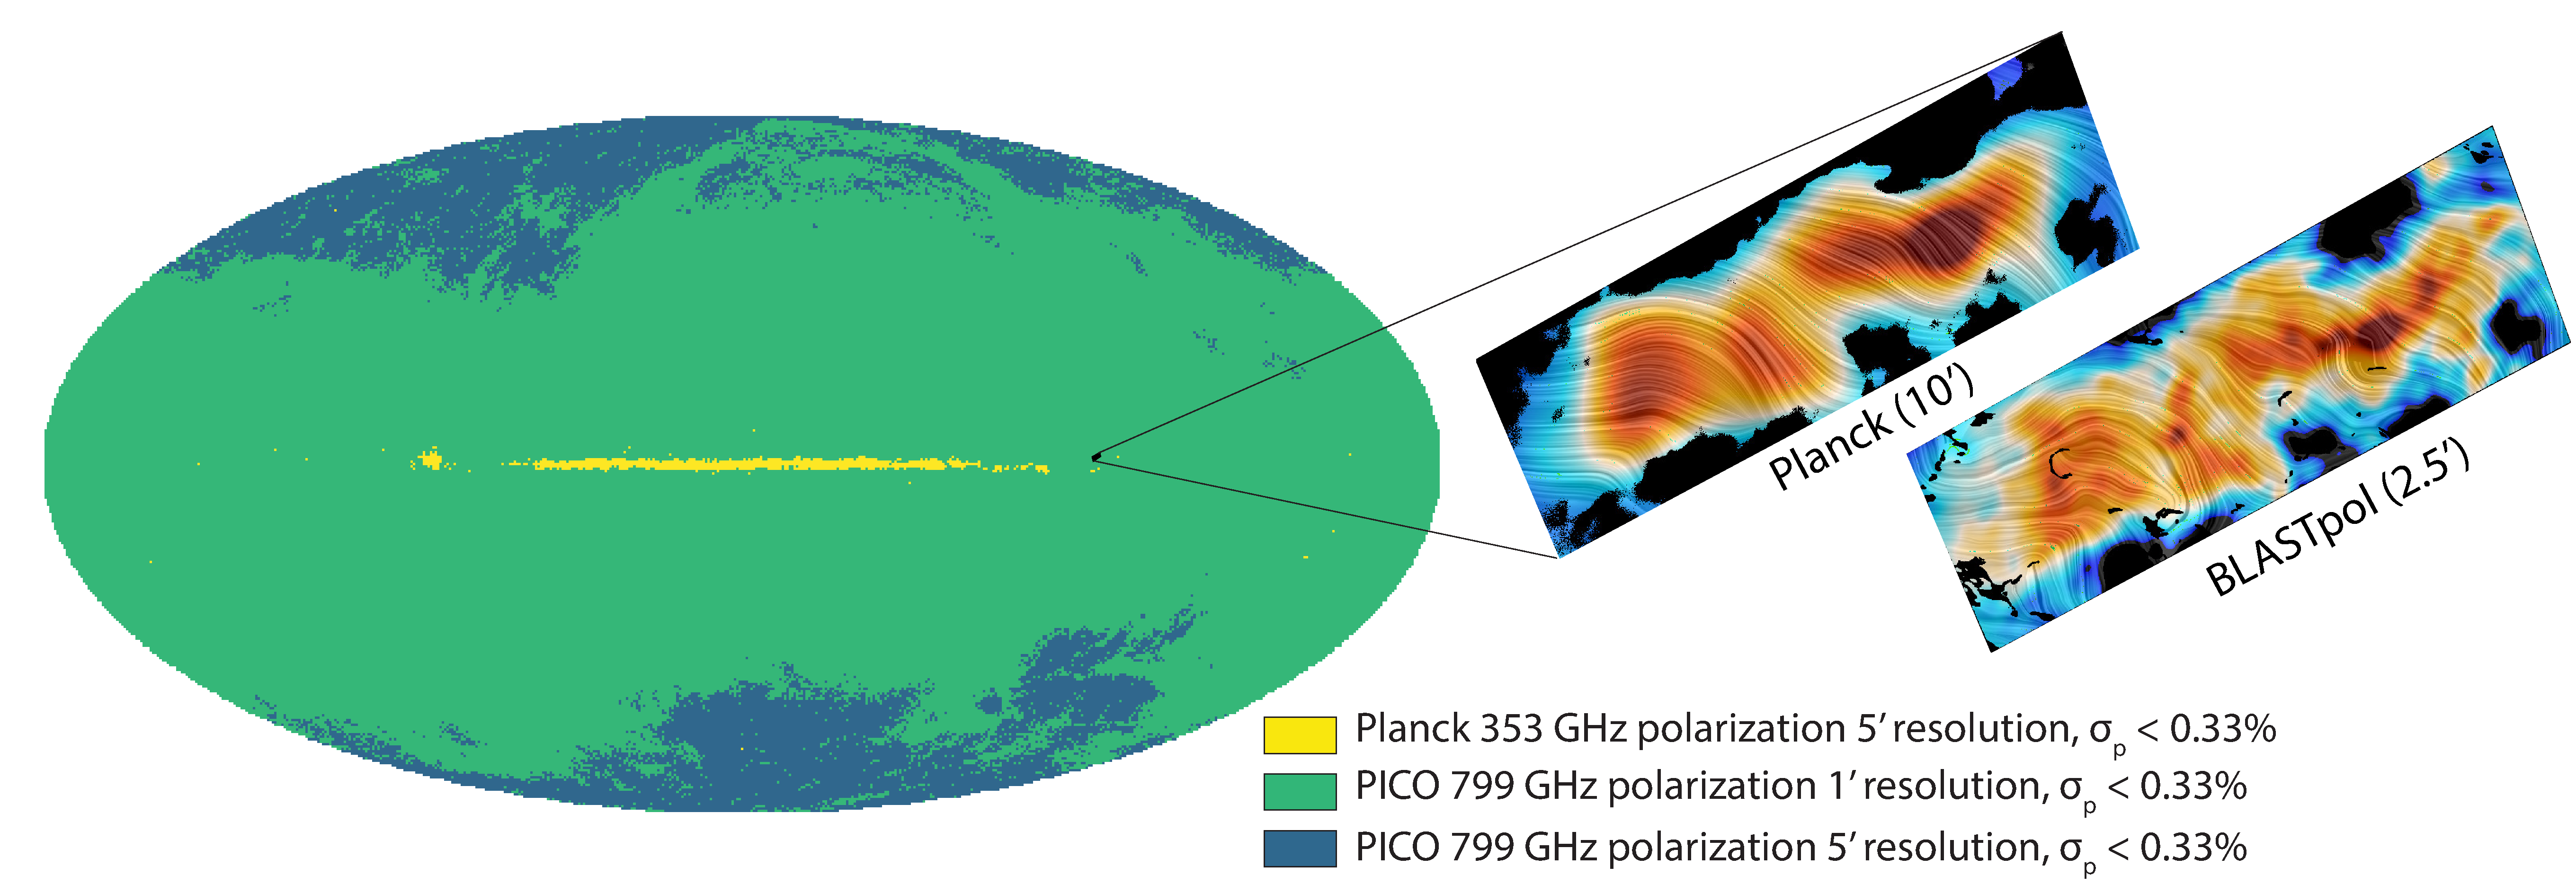
\includegraphics[width=6in]{galsci_fig.pdf}
    \caption{At 799 GHz, PICO will map nearly the entire sky at 1$^{\prime}$ resolution. As an example of the current state-of-the-art, Planck (10$^{\prime}$) and BLASTpol (2.5$^{\prime}$) maps of the Vela C region are shown \citep{Fissel2016}. These observations will enable PICO to characterize magnetized turbulence from the diffuse ISM down to dense star forming cores.}
    \label{fig:allsky}
\end{figure}

{\bf Dust Physics}\\
Strong extinction features at 9.7 and 18\,$\mu$m indicate much interstellar dust is in the form of amorphous silicates while features at 2175\,\AA, 3.3\,$\mu$m, and 3.4\,$\mu$m attest to abundant hydrocarbons. It is unknown, however, whether the silicate and carbonaceous materials coexist on the same grains or whether they are segregated into distinct grain populations. If there are indeed multiple grain species, this will induce additional challenges for modeling the emission from interstellar dust in both total intensity and polarization at levels relevant for B-mode science \citep{Hensley2018}.

Spectropolarimetry of dust extinction features found robust polarization in the 9.7\,$\mu$m silicate feature \citep[e.g.,][]{Smith2000}, indicating that the silicate grains are aligned with the interstellar magnetic field. In contrast, searches for polarization in the 3.4\,$\mu$m carbonaceous feature have yielded only upper limits, even along sightlines where silicate polarization is observed \citep{Chiar2006,Mason2007}. These data suggest that most of the silicate and carbonaceous materials do not exist on the same grains. However, these studies are limited to only a few highly-extincted sightlines that may not typify the diffuse ISM.

At odds with the spectropolarimetric evidence from dust extinction, current measurements of the polarization fraction of the far-infrared dust emission with {\it Planck} \citep{Planck_Int_XXII} and BLASTPol \citep{Ashton2018} betray little to no frequency dependence, as would be expected if two components with distinct polarization properties were contributing to the total emission. However, current uncertainties are relatively large and the data with $\nu > 353\,$GHz are from high density sightlines that may not be representative of the diffuse ISM. With great polarization sensitivity even in diffuse regions, PICO will provide a definitive test of the two component paradigm.

To assess PICO's ability to discriminate quantitatively, we employ the analytic two component dust mode of \cite{Meisner2015} which provided a better fit to IRAS and {\it Planck} data than one component models. 

Applying the noise estimates from PICO, 1000 simulations were run for different combinations of polarization fractions of the two components in this model. Only frequency channels 107 GHz and above were used, and the simulated data were binned to the 7.9$^\prime$ beam of PICO's 107 GHz channel. Based on the variance of the simulation results, PICO can determine the intrinsic polarization fractions of the two components to a precision of 1-2\%. PICO will therefore be able to validate or reject state-of-the-art dust models \citep[e.g.][Hensley \& Draine, in prep]{Guillet2018} and test for the presence of additional grain species with distinct polarization signatures, such as magnetic nanoparticles \citep{Draine2013}.


{\bf Are Magnetic Fields Responsible For Low Star Formation Efficiency?}\\
Stars form out of dense, gravitationally unstable regions within molecular gas clouds. The efficiency of this conversion from molecular gas to stars is very low, due to regulation from supersonic turbulent gas motions, magnetic fields, and feedback from young stars \citep{McKee2007}. 
Magnetic fields may play an important role in slowing the process of star formation by inhibiting movement of gas in the direction perpendicular to the field lines.  Observations to date suggest that the outer envelopes of clouds can be supported against gravity by magnetic fields, but in dense cores gravity tends to dominate, and so these dense structures can collapse to form stars \citep{Crutcher2010}.


On larger scales, the formation of gravitationally unstable clouds is regulated by the flow of diffuse material into the molecular phase, a process that is mediated by magnetized turbulence in the low-density ISM. Structure formation in the diffuse ISM is poorly understood, but as a precursor to star formation it is crucial to understand what drives molecular cloud formation. Recent observations suggest that the structure of the diffuse medium is highly anisotropic, and strongly coupled to the local magnetic field \citep{Clark:2014, Clark:2015, Kalberla:2016, KalberlaKerp:2016}.

However, the degree to which magnetic fields affect the formation of molecular clouds as well as stars within these clouds is poorly constrained, in large part due to the difficulty of making detailed maps of magnetic fields in the interstellar medium.


{\em Formation of Stars within Magnetized Molecular Clouds}\\
With full-sky coverage and a best resolution of 1.1\arcmin~PICO will be able to map all molecular clouds with better than 1\,pc resolution, out to a distance of 3.4\,kpc.  Extrapolating from the Bolocam Galactic Plane Survey \citep[BGPS,][]{EllsworthBowers2015}, we expect 
PICO to make highly detailed magnetic field maps of over 2,000 molecular clouds with thousands to hundreds of thousands of independent measurements per cloud. 

Our goal is to constrain both the strength of the magnetic field, $B$, within these clouds, as well as the energetic importance of the field compared to self-gravity (parameterized by the mass-to-flux ratio $\mu$) and turbulence (parameterized by the Alfv\'{e}n Mach number $\mathcal{M}_A$) as a function of density. 
To measure these quantities we will apply a series of established polarization analysis techniques:
(1) characterizing the relative orientation of cloud structures and the magnetic field \citep{Soler2013,Chen2016,Soler2017,Planck:XXXV}; (2) probability distributions functions of polarization measurables \citep{Fissel2016, King2018}; (3) comparison between the magnetic field and velocity gradient directions \citep{GonzalezCasanova2017,Yuen2017,Lazarian2018}; and (4) measuring the angular dispersion of the magnetic field  \citep{Davis1951,Chandrasekhar1953, Hildebrand2009,Houde2009}.
By applying all four techniques to both PICO observations and synthetic polarization maps made from ``observing'' numerical simulations of star formation, we will quantitatively compare theory and observations. PICO's large number of frequency bands will be used to better modeling the temperature and polarization efficiency of the cloud dust  \citep{Andersson2015}, which can then be used to generate more realistic generation of synthetic observations from simulations for comparison with PICO observations \citep{Seifried2018}. We can then compare the observed magnetization levels derived from the PICO observations to the levels of turbulence derived from molecular gas surveys (e.g.:~\citealt{EllsworthBowers2015, Miville-Deschenes2017}), and the efficiency of star formation, measured from near and far-IR observations of dense cores and protostars with {\em Herschel}, {\em Spitzer}, and {\em WISE}. 

{\bf PICO's ability to map thousands of clouds is not possible with any other current or proposed polarimeter}. {\em Planck}, for example, was only able to map 10 nearby clouds to a similar level of detail \citep{Planck:XXXV}. This large sample of clouds is crucial because dust polarization observations are sensitive to only the magnetic field projected on the plane of the sky, and therefore polarization maps will look very different for molecular clouds observed at different viewing angles.  {\bf By observing thousands of molecular clouds PICO will determine the role of magnetic fields in star formation as a function of cloud age and mass.}


{\em Formation of Magnetized Molecular Clouds from The Diffuse Interstellar Medium}\\
Structure formation in the diffuse ISM is a key area of study motivating observations across the electromagnetic spectrum. PICO's observations will complement recently completed high dynamic range neutral hydrogen (\HI) surveys, such as \HI4PI \citep{HI4PI:2016} and GALFA-\hi \citep{Peek:2018}, as well as planned surveys of interstellar gas, most prominently with the Square Kilometer Array (SKA) and its pathfinders. One of the open questions in diffuse structure formation is how gas flows within and between phases of the ISM. A planned all-sky absorption line survey with SKA-1 will increase the number of measurements of the ISM gas temperature by several orders of magnitude \citep{McClure-Griffiths2015}. Quantitative comparisons of the ISM temperature distribution from SKA-1 and estimates of the magnetic field strength and coherence length scale from PICO will elucidate the role of the magnetic field in ISM phase transitions.

Despite its importance, a comprehensive understanding of the magnetized diffuse ISM is challenging because of its diverse composition, its sheer expanse, and the multi-scale nature of the physics that shapes it. How are matter and energy exchanged between the diffuse and dense media? This question must be addressed by measuring the properties of the magnetic field over many orders of magnitude in column density. PICO is unique in its ability to do this in the diffuse ISM. \textit{Planck} achieved measurements of the diffuse sky at 60$^\prime$ resolution, resulting in $\sim$30,000 independent measurements of the magnetic field direction in the diffuse ISM.  With 1.1\arcmin~resolution PICO will expand the number of independent polarization measurements in the diffuse ISM to $\sim$86,000,000. This will allow us to robustly characterize turbulent properties like $M_A$ across a previously unexplored regime of parameter space. 

{\bf Legacy Science}\\
PICO will also produce legacy datasets that will revolutionize our understanding of how magnetic fields influence physical processes ranging from planet formation to galaxy evolution.  For 10 nearby clouds (d $<$\,500 parsecs) PICO will resolve magnetic fields on the crucial 0.1\,pc size scale associated with dense cores and filaments, and observe how the magnetic fields on these scales directly influence the formation structure of cores.  By comparing the orientation of the core-scale magnetic field with respect to the orientation and sizes of protoplanetary disks, PICO will directly test whether there is evidence that magnetic breaking inhibits the growth of protoplanetary disks \citep{allen_2003,li_2014}. 

On larger scales PICO's tens of millions of independent measurements of magnetic field orientation from will allow us to directly probe magnetized turbulence with in unprecedented detail, allowing us to study how magnetic fields are generated through turbulence and large scale gas motions \citep{Xu_2018}.   The magnetization levels of the also dramatically change key processes in the diffuse ISM, including heat transport \cite{Lazarian:2006}, streaming of cosmic rays \cite{Lazarian:2016}, magnetic reconnection \cite{Lazarian_Vishniac:1999} etc.

Finally, PICO observations will create detailed magnetic field maps of approximately 70 nearby galaxies, with more than 100 measurements of magnetic field direction per galaxy.  These observations will be used to study the turbulence on galactic scales, determine whether the magnetic fields of the Milky Way in the Diffuse ISM are consistent with other galaxies, and directly study how interaction between large scale magnetic fields, turbulence, and feedback from previous generations of star galaxy evolution and star formation efficiency.

For  all of the science described in PICO will provide crucial large number statistics all-sky coverage, and will bridge the spatial scales covered by its predecessor {\em Planck}~and high resolution ground based telescopes like ALMA.



%\bibliographystyle{aasjournal}
%\bibliography{galsci.bib}

\end{document}

%\begin{figure}[!htb]
%\centering
%\includegraphics[width=4cm]{images/example}
%\caption{example}
%\label{fig:im_3}
%\end{figure}


\subsection{Legacy Science}
\documentclass[../PICOReport.tex]{subfiles}

\begin{document}
blah

\begin{figure}[!htb]
\centering
\includegraphics[width=4cm]{../images/example}
 
\label{fig:im_example}
\caption{example}
\end{figure}


\end{document}

\subsection{Foregrounds}

\documentclass[PICOReport.tex]{subfiles}

\begin{document}

%Enumerate the various signals in polarization. Use the frequency band + signals figure. The challenge is to dig out the faintest of all signals, the one due to $r$. This sets the tone for the entire 'signal decomposition' or 'component separation'.  Removing the galactic signal to unmask $r \lesssim 0.001$ is a challenge for all future experiments searching for $r$ at that level, and is a strong advantage of a space platform. The physics of galactic signals suggests complexities in their combined emission properties; the level of this complexity is not known. } 

Diffuse Milky Way emissions dominate the sky's polarized intensity on the largest angular scales; see Figures~\ref{fig:clbb} and ~\ref{fig:pico-channels-and-fg}. Even though their levels decrease when considering smaller angular scales, they are still considerably brighter 
near the \ac{IGW} peak at $\ell=80$ when averaging over 60\% of the sky. 
Even in the cleanest, smaller patches of the sky, far from the galactic plane and thus relatively low in galactic emissions, their levels are expected to be substantial relative to the \ac{IGW} for $r \lesssim 0.01$, and dominate it for $r \lesssim0.001$. Separating the cosmological and Galactic emissions signal, also called foreground separation, together with control of systematic uncertainties are {\it the} challenges facing any next decade experiment attempting to reach these levels of constraints on $r$.

\begin{figure}
\includegraphics[width=0.49\textwidth]{images/sensitivity_vs_frequency_Jun29th_2018_large.pdf}
\includegraphics[width=0.49\textwidth]{images/sensitivity_vs_frequency_Jun29th_2018_2deg.pdf}
\vspace{-0.1in}
\caption{Polarization $BB$ spectra of Galactic synchrotron and dust, compared to CMB polarization $EE$ and $BB$ spectra of different origins for two values of $r$ and for two ranges of angular scales: large $\ell \leq 10$ corresponding to the reionization peak (left panel), and intermediate $50 \leq \ell \leq 150$ corresponding to the recombination peak (right panel). The location and sensitivity of the 21 PICO frequency channels is shown as vertical bands. (The color scheme is explained in Section~3.2.) }
\label{fig:pico-channels-and-fg}
\end{figure}

The foreground separation challenge would be easily surmountable if the Galactic emissions were already precisely characterized, or were known to have simple, fittable spectral emission laws. But neither is true. Until recently, the spectrum of Galactic synchrotron emission, arising from free electrons spiraling around Galactic magnetic fields, was modeled as a power law $I_{\rm sync} \propto \nu^{\alpha},$ with $\alpha \simeq -1$ (in brightness units). The spectrum of Galactic dust emission, arising from emission by Galactic dust grains, was modeled as $I_{\rm dust} \propto \nu^{\beta} B_\nu(T_{\rm dust}),$ where $\beta \simeq 1.6$, $T_{\rm dust} \simeq 19$\,K, and $B_\nu(T)$ is the Planck function; this is referred to as `modified black body emission'. In principle, an experiment that had 6 frequency bands could determine the three emission parameters as well as the three amplitudes corresponding to that of dust, synchrotron, and the CMB. However, WMAP and Planck observations have shown that neither emission law is universal and that spectral parameters vary with the region of sky \comor{is this true? is there evidence from Planck; add references} (thus that the values given above are valid only as averages across the sky). Also, while both emission laws are well-motivated phenomenological descriptions, the fundamental physics of emissions from grains of different materials, sizes and temperatures, and of electrons spiraling around magnetic fields implies that these laws are not expected to be exact, nor universal. 

We know that we don't know enough about synchrotron and dust emission. We know even less about the polarization level of 'anomalous microwave emission', an excess of dust emission at frequencies between 10 and 100~GHz, and of infra-red sources. Depending on reasonable levels of polarization assumed their contributions to the total polarized signal may be appreciable or negligible (for $r\lesssim 0.001$)~\citep{??}.  

Faced with these uncertainties, but also with the opportunity provided by a platform that can host a broad range of frequencies -- ground-based experiments are limited to several atmospheric windows and to frequencies of less than 300~GHz -- PICO is designed with 21 frequency bands between 21 and 800 GHz; see Figure~\ref{fig:pico-channels-and-fg} and Table 3.2. This is the broadest frequency lever arm proposed by any imaging instrument to characterize and enable separation of Galactic emissions. 

Foreground uncertainties, and the level of fidelity required in their characterization, also compel a transition in the way we assess and forecast the performance of a future experiment. We can no longer impose specific models upon the data; \comor{several publications have demonstrated that deviations between assumed models' parameters and the real sky could give rise to biases in $r$ that are larger that future goals~\citep{which??}. Al, make this more concrete?} Rather, the data collected should provide information to constrain Galactic emissions with sufficient accuracy. For PICO we use the approach that has become the `gold standard' in the community. In this approach we simulate sky maps that are constrained by available data, but otherwise have a mixtures of foreground properties, observe these maps just like a realistic experiment will do, and then apply foreground separation techniques to separate the Galactic and CMB emissions. We also provide forecasts using other techniques that use analytic calculations to estimate the efficacy of foreground separation, or others in which the simulated sky map is assumed to have specific Galactic emission models, which are then being fitted. 

%\comor{now need to connect to the next paragraphs} As we show below, the PICO broad frequency coverage, coupled with high sensitivity enables studying the sky using the PICO data themselves rather than assuming what the sky is, and fitting our models to these assumptions. 

%%%%%%%%%%%%%%%%%%%%%%%%%%%%%%%%%%%
\subsubsection{PICO Foreground Separation Methodology}
%%%%%%%%%%%%%%%%%%%%%%%%%%%%%%%%%%%

\noindent{\bf Sky Maps} \hspace{0.1in} For assessing the efficacy of foreground separation with PICO we used 8 different full sky models. All models were consistent with and constrained by available data and uncertainties from WMAP and \planck . The range of models included one test case that had a very simple realization of foregrounds, and others with varying degree of complexity including spatially varying spectral parameters and along the line of sight, anomalous microwave emission \comor{up to 2\%} polarized, dust polarization that rotates slightly as a function of frequency because of projection effects, or dust spectral energy distribution that departs from a simple modified blackbody. All foreground maps are generated at native resolution of 6.8 arcmin pixels~\citep{healpix}. They are generated using PySM and/or PSM codes~\citep{??}.   Distinctly different realizations of the sky are allowed by current data, as demonstrated by Figure~\ref{fig:skymodels}. \comor{ Karl, More details of the models are available at~\citet{foregroundappendix}.}

For each of the 8 models we added CMB signals in both intensity and polarization matching a $\Lambda$CDM universe. The $BB$-lensing signal matched the level of 85\% delensing forecasted for PICO. Each of these sky models had 100 different realization of the PICO CBE noise levels; 50 realizations had no \ac{IGW} signal and 50 others had a level of $r=0.003$. 

\vspace{0.1in}
\noindent{\bf Foreground Separation} \hspace{0.1in} The sky models were analyzed with a variety of techniques which are based on two broad categories: correlation methods, which exploit the fact that foreground emission is strongly correlated from frequency to frequency, but uncorrelated with the CMB, and parametric methods, which model the sky emission using specific (parametric) emission laws, and use spectral fits in independent pixels or sky regions to infer the amplitude and spectral parameters of each of the components in the sky. Correlation methods include SEVEM, and variants of the \ac{ILC} algorithm, such as the needlet-space \ac{ILC} (NILC) and a version generalised to multidmensional components (GNILC). Parametric methods include the Commander algorithm.

%\vspace{0.1in}
%\noindent{\bf Acknowledged Limitations} \hspace{0.1in} The level of effort supported 

%%%%%%%%%%%%%%%%%%%%%%%%%%%%%%%%%%%
\subsubsection{Results and Discussion}
%%%%%%%%%%%%%%%%%%%%%%%%%%%%%%%%%%%

\begin{figure}
\hspace{-0.1in}
\parbox{3.0in}{\centerline {
\includegraphics[width=3.0in]{images/soumen_NILC_foregrounds_93.png}}}
\hspace{0.25in}
\parbox{3.0in}{
\caption{Caption . . . \dotfill
\label{fig:nilc}}}
\vspace{-0.1in}
\end{figure}

%\begin{figure}
%\hspace{-0.1in}
%\parbox{4.0in}{\centerline {
%\includegraphics[width=0.6\textwidth]{images/mathieu_GNILC_foregrounds.png}}}
%\hspace{0.in}
%\parbox{2.0in}{
%\caption{Caption . . . 
%\label{fig:gnilc} } }
%\vspace{-0.1in}
%\end{figure}

\begin{figure}
\hspace{-0.1in}
\parbox{4.5in}{\centerline {
\includegraphics[width=4.5in]{images/commander_foregrounds_BB.png}}}
\hspace{0.in}
\parbox{2.0in}{
\caption{Caption . . .  \dotfill
\label{fig:commander}}}
\vspace{-0.1in}
\end{figure}


The most important lesson arising from our exercise is that more work is required to ascertain that levels of $r \lesssim 0.001$ can be determined robustly on the largest angular scales, that is from the reionization peak.  Figure~\ref{fig:nilc} shows results from the NILC analysis. For several of the sky models the power spectra of the residual level of foregrounds -- that is the level of foregrounds remaining in the map after foreground separation -- is below the cosmological \ac{IGW} level with $r =0.003$. For a minority of the models, the residual is higher at $\ell \lesssim 20$. Results from GNILC, shown in Figure~\ref{fig:gnilc}, are similar. In all cases, the analyses are carried out using 60\% of the sky, the results shown are from one realization, and that no further optimization of the basic foreground separation technique has yet been applied. 

More work is also required to understand the necessary span of frequencies required. Figure~\ref{fig:psm_mr} shows that removing several of PICO's frequency bands, in this case the three highest, significantly biases the extracted $BB$ power spectrum, particularly at the lowest $\ell$ values. This result should not be interpreted as conclusively demonstrating that a frequency span up to 800 GHz has been proven to be essential. At this point of time, different input sky models, coupled to different foreground separation techniques may yield different results. Rather, the conclusion is that further improvement in our modeling and analysis is required. 

While these initial results are encouraging, as they suggest that PICO's frequency coverage and sensitivity may be adequate for this level of $r$, more work should be invested to gain complete confidence that this and lower levels of $r$ can be extracted. This work includes, but not limited to: running more realizations; is ahead to 

Reducing the sky area used to 50 or




\noindent{\bf Required Frequency Span} \hspace{0.1in}


%%%%%%%%%%%%%%%%%%%%%%%%%%%%%%%%%%%
\subsubsection{Discussion}
%%%%%%%%%%%%%%%%%%%%%%%%%%%%%%%%%%%


\end{document}

%\begin{figure}[!htb]
%\centering
%\includegraphics[width=4cm]{images/example}
%\caption{example}
%\label{fig:im_3}
%\end{figure}


%The baseline design of PICO has 21 channels observing the sky in the 20\,GHz to 800\,GHz frequency range (Fig.~\ref{fig:pico-channels-and-fg}). By analysing how the total emission varies across frequency bands, one can infer the detailed emission properties of the various emission components, form linear combinations of the observations that maximise the contribution of a component of interest while minimising contamination by the others and by instrumental noise, and understand the properties of the foregrounds to evaluate potential residuals in the CMB B-mode map. Various such techniques have been successfully used in previous CMB observations such as those of the Planck mission. Building on this existing expertise, we have carried out map based simulations within a ``data challenge'' framework to assess the capacity of PICO to measure the main signal of interest (CMB primordial B-modes). In this process one group prepares sets of simulated maps for different models of foreground emission of varying complexity from optimistic to pessimistic, which are placed in a shared area. These are then re-analyzed by multiple individuals and groups employing various different component separation algorithms.



\subsection{Systematic Errors}
\documentclass[PICOReport.tex]{subfiles}

%\newcolumntype{L}[1]{>{\raggedright\let\newline\\\arraybackslash\hspace{0pt}}m{#1}}
%\newcolumntype{K}[1]{>{\raggedright\centering\arraybackslash}m{#1}}

\begin{document}
Aside from control of foregrounds, the most compelling reason to observe the CMB from space is the opportunity for excellent control of systematic errors that affect CMB measurements from any platform.  
The L2 environment offers excellent stability as well as the ability to observe large fractions of the sky on many time scales without interference from the Sun, Earth, or Moon.
The redundancy of observations allows the checking of consistency of results and an improved ability to calibrate and to correct systematic errors in post-processing analysis.

As of today, there is a clear path to demonstrate that state-of-the-art technology and data processing can take advantage of the L2 environment and control systematic errors to a level that enables the science goals of PICO. 

A rich literature investigates the types of systematic errors due to the environment, the instrumentation, observation strategies, and data analysis that confound the polarization measurement by creating a bias or an increased variance\cite{hu03,shimon2008,yadav2010}. 
Every measurement to date has  reached a systematic error limit, and have advanced many sophisticated techniques to mitigate systematics, finding both new technological solutions and new analysis techniques.
As an example, the BICEP's systematics limited it to r=0.1\cite{Takahaski2010} while through additional effort within the program, BICEP2 achieved a systematics limit of r=6$\times$10$^{-3}$\cite{BICEP2_III}).
In the near term, the ground based and suborbital CMB community will continue to develop new techniques in handling systematics, particularly in developing the CMB-S4 project.

All prior on-orbit measurements of CMB polarization were limited by systematic errors until an in-depth study of the systematics was performed and the post-processing data analysis suppressed them\cite{Bennett13,planck2016_xlvi,Planck2018_I}. 
Paricularly we note Fig. 3 of the Planck legacy paper which indicates Planck's systematic error limits on the polarization power spectral measurements.
Recently studied space missions, such as EPIC-IM, LiteBird and  \core, have placed
systematic error mitigation at the forefront of the case for their
mission and have developed tools and strategies for estimating and mitigating these\cite{hazumi2012,wallis2017,Natoli2018}.

End-to-end simulation of the experiment is an essential tool,
including realistic instabilities and non-idealities of the spacecraft,
telescope, instrument and folding in data post-processing techniques
used to mitigate the effects.  Systematics are coupled with the
spacecraft scan strategy, and the details of the 
data analysis pipeline.  

\subsubsection{List of Systematics}
The systematic errors faced by PICO can be categorized into three broad categories: 
1) Intensity-to-polarization leakage, 2) stability, and 3)
straylight and are listed in Table \ref{tbl:SystematicsList}.  
These were prioritized for further study using a risk factor assessed by the working group.  
The risk factor incorporates the working group's assessment of how mission-limiting the effect is, how well these effects are understood by the community and whether mitigation techniques exist.  

The working group's three highest risk systematic errors were studied further and are discussed in subsections below.  The PICO team used 
 simulation and analysis tools developed for Planck\cite{plank2015_xii_focalplane} and \core, adapting them for PICO.

We note that many of the systematics could be mitigated further through the use of polarization modulation such as a half-wave plate or a variable phase delay modulator.  
For the purposes of the cost constraints of PICO, we investigated mitigation techniques that do not require a modulator.  

\begin{table}[h!]
\centering
\scriptsize
 \begin{tabular}{p{3.3cm} p{0.5cm} p{4.2cm} p{4.2cm} p{4.2cm}}
 \hline
\textbf{Name} & \textbf{Risk}&\textbf{Description} & \textbf{State-of-the-art} & \textbf{Additional Mitigation Needed} \\
 \hline
\textbf{Leakage}& &\\
Polarization Angle Calibration\dotfill& 
5&
Uncertainty in polarization calibration leaks E$\to$B.
& 
Knowledge of astrophysical calibrators to 0.3$^\circ$\citet{Aumont+2018}; ground measurement to 0.9$^\circ$ reconstruction to 0.2$^\circ$ using $TB$ and $EB$ demonstrated by \planck\citet{Planck_Lowell}
& 
See Sect.~\ref{sec:angle} for discussion.
\\
 Bandpass Mismatch\dotfill&
 4& 
 Edges and shapes of the the spectral filters vary from detector to detector. leaks T $\to$ P, P $\to$ P if the source's bandpass differs from calibrator's bandpass\cite{Hoang_2017} & Precise bandpass measurement\cite{Pajot_2010};
SRoll algorithm\cite{Planck_Lowell}; filtering technique\cite{CORE_systematics};  additional component solution (see Banerji\& Delabrouille in prep). &
State-of-the-art meet requirements.
   \\
Beam mismatch\dotfill& 
4&
Beam shapes differ between detectors that are combined to reconstruct polarization; leaks T $\to$ P, P $\to$ P
& See Sect.~\ref{sec:angle} & State-of-the-art meet requirements.\\
Time Response Accuracy and Stability\dotfill&
4&
Uncertainty of detector in time constants (measurement errors, time variability) biases polarization angle, pointing and beam size. In a constant spin-rate mission (\pico) is degenerate with the beam shape. leaks T$\to$P, P$\to$P&
On-orbit reconstruction of time response to 0.1\% across a wide signal band\cite{planck2013_vii}, residuals corrected as part of beam and map-making algorithm\cite{Planck_Lowell}.
& State-of-the-art meet requirements.
\\
Readout Cross-talk\dotfill& 
4&
Power in one detector leaks into other detectors
&
\planck's high-impedence bolometers with crosstalk measured at the level of 10$^{-3}$ did not impact CMB polarization science\cite{Planck_Lowell}.  Cross-talk low-impedence bolometers measured at XXX.
&
State-of-the-art meets requirements.
\\
Chromatic beam shape\dotfill&
4&
Beam shape is a function of source SED: measured using a planet, used to build a window function to correct CMB power spectrum.
&
\planck\ simulations and parameterization as part of the likelihood.
&
Should be further investigated in Phase A of a mission using physical optics simulations.  
\\

Gain mismatch\dotfill&
3&
Relative gain between detectors that are combined to reconstruct polarization; error leaks T$\to$P &
mission-average relative calibration demonstrated to 10$^{-4}$ to 10$^{-5}$ level \cite{Planck_Lowell}
&
State-of-the-art measurement of mission-average gain meets requirements; Sect.~\ref{sec:gain} describes effects of stability in time in relative gains.  
\\


Cross-polarization\dotfill&
3&
Q$\to$U rotation by the optical elements of the instrument.
&
Degenerate with polarization gain calibration.
&
State-of-the-art meets requirements.
\\
\hline 
\textbf{Stability} & & \\
Gain Stability\dotfill& 
5&
Time-variation of detector gain due to time variability of detector heat sink temperature variations and optical loading.
& 
Reconstruction of time variability of gain to 0.2\% in \planck\cite{Planck_Lowell}.
&
See Sect.~\ref{sec:gain}; Gain fluctuations in \pico\ on the level of XXX\% on time scales of YYY can be corrected in post-processing.
\\
Pointing jitter\dotfill&
3&
Random pointing error mixes T, E and B at small angular scale
&
Pointing reconstruction in \planck\ to XXX arcsec.
&
State-of-the-art meets requirements.
\\

\hline
\textbf{Straylight}& & \\
Far Sidelobes\dotfill& 
5&
Pickup of Galactic signals at large angles from the main beam axis; Spillover can be highly polarized.
& 
\planck\ validated straylight model in anechoic chamber to -80~dBi\cite{Tauber2010}.
&
Design of optical system and baffling, informed by telescope straylight simulations. See Sect.~\ref{sec:fsl} for a study of beams calculated with a physical optics code for the \pico\ telescope and simulated Galactic pickup during the reference mission.\\
 \hline
\textbf{Other} \\
Residual correlated cosmic ray hits\dotfill&
3 &
detectors experience correlated cosmic ray hits below detection threshold resulting in misestimated noise covariance.
&
\planck/HFI found the 5\% percent noise correlation due to this effect did not impact results\cite{Planck_Lowell}. 
&
State-of-the-art detector design to reduce cosmic ray cross-section; State-of-the-art analysis techniques (accounting for correlated noise) meet requirements.
\\
\hline
 \end{tabular}
\caption{\label{tbl:SystematicsList} Systematic errors expected in \pico's measurement of CMB polarization.  The risk level was scored from 1 to 5 based on the study team's assessment.  Those systematic errors found to be most likely to impact \pico\ are described further in the text.}
 \end{table}

\subsubsection{Absolute polarization angle calibration}
\label{sec:angle}

The rotation of the CMB polarization can have different causes,
including 1. a birefringent primordial Universe, or a Faraday rotation
due a primordial magnetic field \citep{Pogosian+2018}, 2. birefringent
foregrounds, or interaction with the Galactic magnetic field,
3. systematic effects in the instrument, and in particular an error on
the actual direction of polarization measured by each detector.  
While the first two sources create a rotation that may depend on scale,
position and/or frequency, the latter depends mainly on
the detector considered. 

A rotation {\prang} of the direction of polarization mixes the $Q$ and $U$ Stokes parameters via
$Q\pm iU \longrightarrow e^{\mp i 2 \prang} (Q\pm iU)$
and thus mixes the the power spectra and their correlations as illustrated in Fig.~\ref{fig:rot_bb_tb_eb}.
% via (assuming the rotation to be independent on scale and location)
%\begin{subequations}
%\begin{align}
%C^{TT}_\ell &\longrightarrow & C^{TT}_\ell                                             &= & C^{TT}_\ell \\
%C^{TE}_\ell &\longrightarrow & \cos 2\prang\  C^{TE}_\ell                                &\sim & \left(1 - 2\prang^2\right)\ C^{TE}_\ell \\
%C^{EE}_\ell &\longrightarrow & \cos^2 2\prang\  C^{EE}_\ell + \sin^2 2\prang\  C^{BB}_\ell &\sim & C^{EE}_\ell - 4\prang^2\ \left(C^{EE}_\ell - C^{BB}_\ell\right) \\
%C^{BB}_\ell &\longrightarrow & \sin^2 2\prang\  C^{EE}_\ell + \cos^2 2\prang\  C^{BB}_\ell &\sim & C^{BB}_\ell + 4\prang^2\ \left(C^{EE}_\ell - C^{BB}_\ell\right)\\
%C^{TB}_\ell &\longrightarrow & \sin 2\prang\  C^{TE}_\ell                                &\sim & 2\prang\  C^{TE}_\ell \\
%C^{EB}_\ell &\longrightarrow & \sin 2\prang \cos 2\prang \left(C^{EE}_\ell -  C^{BB}_\ell\right)  &\sim & 2\prang\ \left(C^{EE}_\ell -  C^{BB}_\ell\right)
%\end{align}
%\end{subequations}


%------------------------------------------------------------------------------------------
\begin{figure}[htb]
\includegraphics[width=0.8\textwidth]{images/PICO_rotate_eb3_v0.\suffix}
\caption{\label{fig:rot_bb_tb_eb} Effect of a rotation of the angle of polarization, assuming the Planck 2018 $\Lambda$-CDM best fit model \citep{Planck2018_VI} with $\tau=0.054$ and expected \pico\ noise performance, assuming perfect delensing.}
\end{figure}
%------------------------------------------------------------------------------------------
%
%------------------------------------------------------------------------------------------
%\begin{figure}[htb]
%\includegraphics[width=0.40\textwidth]{images/PICO_sens2_v0_F5p0_f0p5_n0p62_k4_a1p0_2_4000.\suffix}
%\includegraphics[width=0.40\textwidth]{images/PICO_sens2_v0_F15p0_f0p5_n0p62_k4_a1p0_2_4000.\suffix}
%\caption{\label{fig:rot_sens_0} Upper panels: signal to noise ratio of the polarization angle {\prang} measurement
%by $EB$ (blue lines), $TB$ (green lines) and $BB$ (red lines), assuming either no delensing (solid lines) 
%or perfect delensing (dashes); the shaded area is $|\prang|/\sigma_\prang < 3$.
%Lower panels: degradation on measurement of $r$, for $r=10^{-2},\ 10^{-3},\ 10^{-4}$ (magenta, orange and cyan lines, respectively),
%either with no delensing (solid lines) or perfect delensing (dashes).
%The underlying cosmology is Planck 2018 $\Lambda$-CDM model (with $\tau = 0.054$), and assuming a polarized noise of rms = $0.62 \mu K.\arcmin$ and power spectrum $(1 + (\ell_{\rm knee}/\ell)^n)$ with $\ell_{\rm knee}=4$ and $n=1$, with the analysis done on the multipole range $[2,4000]$ over a sky fraction $\fsky=0.5$. The beam FWHM$=5\arcmin$ on the \emph{lhs} and $15\arcmin$
%on the \emph{rhs} panels. \EFH{Probably remove this figure and summarize in text.}}
%\end{figure}
%
% \begin{figure*}[htb]
% \includegraphics[width=0.5\textwidth]{fig_efh/PICO_sens2_v0_F15.0_f0.5_n0.62_k4_a1.0_2_4000.\suffix}
% \caption{\label{fig:rot_sens_1} Same as Fig.~\ref{fig:rot_sens_0}, with a FWHM=$15\arcmin$.}
% \end{figure*}
%
%\begin{figure}[htb]
%\includegraphics[width=0.40\textwidth]{images/PICO_sens2_v0_F5p0_f0p5_n0p62_k4_a1p0_20_4000.\suffix}
%\includegraphics[width=0.40\textwidth]{images/PICO_sens2_v0_F5p0_f0p5_n1p86_k4_a1p0_2_4000.\suffix}
%\caption{\label{fig:rot_sens_2} Same as Fig.~\ref{fig:rot_sens_0}, left panels, reducing the multipole range $[20,4000]$ (\emph{lhs}) or with a noise rms multiplied by 3 (\emph{rhs}).\EFH{Probably remove this figure and summarize in text.}}
%\end{figure}
% %
% \begin{figure*}[htb]
% \caption{\label{fig:rot_sens_3} Same as Fig.~\ref{fig:rot_sens_0}, with a noise rms multiplied by 3.}
% \end{figure*}
% %------------------------------------------------------------------------------------------

In Planck, the ground measurements of the detectors orientation had an error of $\pm 0.9\degree$ (rel.) $\pm 0.3\degree$ (abs.) \citep{Rosset+2010}.

The most recent constraints on cosmological birefringence (or systematic rotation) was set in \citet{Planck2016_XLIX}, looking for residual signal in $TB$ and $EB$ spectra, but are dominated by the uncertainties on the detector orientations.

For \pico, the relative rotation of the detectors, could be measured with a good accuracy (a few $0.1\arcmin$ ?, \EFH{refs?}) on the CMB, but the overall rotation is difficult to determine.
Known polarized sources, such as the Crab Nebula, could be used to do that but \citet{Aumont+2018} show that the current uncertainty of $0.33\degree = 20\arcmin$ on the Crab polarization orientation, obtained when combining all the available measurements, 
would not the measurement of tensorial $B$ modes below $r \sim 0.01$ (assuming everything else to be nominal), far from \pico's target.

%Figures \ref{fig:rot_sens_0} and \ref{fig:rot_sens_2} show how the measurement of $r$ by \pico\ is degraded because of an overall rotation of polarization, and how $TB$ and $EB$ can be used to monitor this rotation, assuming that the only source of polarization rotation is instrumental.
%These results are obtained assuming the spectra to have a Gaussian likelihood, with a variance $\propto 1/\fsky$, and ignoring the foreground contributions.

In the absence of other systematics and foregrounds, an unaccounted polarization rotation $\alpha$ of $10\arcmin$ increases
the error bar of $r$ by 30\%, while $EB$, $TB$ and $BB$ spectra can measure a rotation $\alpha$ at 3$\sigma$ when $\alpha \sim 0.07, 0.2$  and $0.9\arcmin$ respectively
 on perfectly delensed maps, and $0.25, 0.9$ and $4.5\arcmin$ on raw maps.

In principle, the technique of using the $TB$ and $EB$ spectra can detect and measure a global polarization rotation error at levels ($~0.1 \arcmin$) well below those affecting $r$ measurements in $BB$ ($> 1 \arcmin$).  However, a future mission should include additional aspects of the measurements of CMB polarization, such as delensing, the interaction with foregrounds, and $1/f$ noise in simulating and assessing the impact of an angle calibration error.

\subsubsection{Gain Stability}
\label{sec:gain}
Photometric calibration is the process of converting the raw output of the receivers into a physically-meaningful quantity, such as thermodynamic temperature or brightness. As CMB receivers are usually linear, this process reduces to the characterization of the \emph{gain factor} $G$:
\begin{equation}
\label{eq:gainStability:Response}
y(t) = G(t) \times T\bigl(\vec{x}(t)\bigr) + n(t),
\end{equation}
where $y(t)$ is the timestream of raw samples produced by the detector, $G(t)$ is the gain factor (which we allow to vary with time), $T$ is the sky temperature observed along direction $\vec{x}(t)$ (which varies with time as the spacecraft spins), and $n(t)$ is a noise term that includes both uncorrelated and correlated noise. It is assumed that the timescale of variation in $G$ ($G / \dot{G}$) is much longer than the typical timescale of variations in $T$: in the case of Planck, this was of the order of several days.

In the case of space CMB experiments, the characterization of $G(t)$ is commonly done using the signal caused by the motion of the spacecraft with respect to the rest frame of the CMB itself. This signal is commonly called the \emph{dipole}, as its most significant contribute is at multipole $\ell=1$. For the PICO concept study, we evaluated the impact of noise in the estimation of $G(t)$ using the tools developed for the Planck/LFI instrument and the CORE mission proposal. The quality of the estimate depends on the noise level of the receiverse, but also on the details of the scanning strategy. The Planck/LFI experiment, because of a poor choice of the scanning strategy parameters (namely, a too slow precession motion), was forced to avoid using one year out of four in the 2015 data release [REF]. We can anticipate that this problem is not expected in PICO, thanks to the significantly faster precession envisaged.

In order to test the impact of calibration uncertainties, we have run the following analysis:
\begin{enumerate}
\item\label{step:gainStability:perfectObservation} We simulated the observation of the sky, assuming four receivers and the nominal scanning strategy. We included both white noise and $1/f$ noise. The sky only contained CMB anisotropies, plus the CMB dipole.
\item\label{step:gainStability:calibration} We ran the calibration code to fit the dipole against the raw data simulated during step~\ref{step:gainStability:perfectObservation}.
\item\label{step:gainStability:imperfectObservation} We simulated again the observation of the sky, but this time we used the values of $G$ computed during step~\ref{step:gainStability:calibration}, which contain errors due to the presence of $n(t)$ and the CMB signal in Eq.~\eqref{eq:gainStability:Response}. The noise in the output map is therefore the sum of the noise in the error on $G$ and the term $n$.
\end{enumerate}
The presence of foregrounds in the sky signal would cause a bias in the estimation of the calibration constants, due to the presence of large scale features in the Milky Way at microwave frequencies. A full data analysis pipeline for PICO should pair the calibration step with the component separation step, following a schema similar to what has been done by the Planck/LFI team for the 2018 data release [CITATION]: the application of the calibration code should be followed by a component separation analysis, and these two steps should be iterated until the result converge to a solution. In this analysis we assume to study the calibration at the last iteration, when the components have already been properly separated.

Results of the simulation are shown in Figures~XXX and YYY. The scanning strategy employed by PICO allows for a much better calibration than in the case of Planck's, thanks to the much faster precession.

\subsubsection{Far Sidelobe Pickup}
\label{sec:fsl}
The main beam (within a few degrees of the axis of beam response) in a CMB mission can be measured to high precision using the planets as compact sources.  Measurement of each detector's response to signals more than a few degrees off axis, which tends to be at a very low level (more than --80dB less than the peak response) but spread over a very large solid angle, is difficult to do pre-launch, and may not be done accurately after launch.  Nonetheless, this far sidelobe can couple bright Galactic signal from many tens of degrees off-axis and confuse it with polarized signal from the CMB off the Galactic plane.  

To evaluate this systematic error, GRASP software\footnote{https://www.ticra.com} was used to compute the \pico\ telescope's pickup over the full sky.  This full-sky beam was convolved with a polarized Galactic signal and a full \pico\ mission scan using the simulation pipeline.  The far sidelibe pickup was estimated to contribute less than XXX to the B-mode angular power spectrum and thus an error in $r$ of YYY.

In a real mission due to the difficulties of measuring this beam, physical optics simulation capabilities must be maintained and validated as well as possible with on-orbit data.

\subsubsection{Key Findings}
Properly modeling, engineering for, and controlling the effects of systematic errors in a
next-generation CMB probe is critical.  In particular we note:
\begin{itemize}
\item The raw sensitivity of the instrument should include enough margin
that data subsets can independently achieve the science goals.
This allows testing of the results in the data analysis and additional
data cuts, if needed.

\item NASA's support of ground-based and suborbital CMB missions will mitigate risk to a future space mission as PICO by continuing to develop analysis techniques and technology for mitigation of systematic errors.

\item In a PICO mission's phase A, a complete end-to-end system-level
simulation software facility would be developed to assist the team in setting 
requirements and conducting trades between subsystem requirements while
realistically accounting for post-processing mitigation.  Any future
CMB mission is likely to have similar orbit  
and scan characteristics to those of PICO, thus there is an opportunity for NASA and
the CMB community to invest in further development of this capability now.
\end{itemize}

\end{document}

%\begin{figure}[!htb]
%\centering
%\includegraphics[width=4cm]{images/example}
%\caption{example}
%\label{fig:im_3}
%\end{figure}


\section{Instrument Implementation (10 pgs)}
\documentclass[PICOReport.tex]{subfiles}

\begin{document}

Telescope, focal plane, cooling, readout 

\end{document}

%\begin{figure}[!htb]
%\centering
%\includegraphics[width=4cm]{images/example}
%\caption{example}
%\label{fig:im_3}
%\end{figure}


\section{Mission Implementation (5 pgs)}
\documentclass[PICOReport.tex]{subfiles}

\begin{document}

To be included: mission architecture, spacecraft and subsystems, orbit, attitude control and determination (Trangsrud)


\end{document}

%\begin{figure}[!htb]
%\centering
%\includegraphics[width=4cm]{images/example}
%\caption{example}
%\label{fig:im_3}
%\end{figure}


\section{Technology Development (4 pgs)}
\documentclass[PICOReport.tex]{subfiles}

\begin{document}

Requirements, planned activities, schedules and milestones, estimated cost (O'Brient?)

\end{document}

%\begin{figure}[!htb]
%\centering
%\includegraphics[width=4cm]{images/example}
%\caption{example}
%\label{fig:im_3}
%\end{figure}


\section{Cost (6 pgs)}
\documentclass[PICOReport.tex]{subfiles}

\begin{document}

cost, risk, heritage (Trangsrud)

\end{document}

%\begin{figure}[!htb]
%\centering
%\includegraphics[width=4cm]{images/example}
%\caption{example}
%\label{fig:im_3}
%\end{figure}


\newpage

\bibliography{mybib}


\begin{acronym}
    %A
    \acro{ACS}{attitude control system}
    \acro{ADC}{analog-to-digital converters}
    \acro{ADS}{attitude determination software}
    \acro{AHWP}{achromatic half-wave plate}
    \acro{AMC}{Advanced Motion Controls}
    \acro{AME}{anomalous microwave emission}
    \acro{ARC}{anti-reflection coatings}
    \acro{ATA}{advanced technology attachment}
    %B
    \acro{BAO}{baryon acoustic oscillations}
    \acro{BRC}{bolometer readout crates}
    \acro{BLAST}{Balloon-borne Large-Aperture Submillimeter Telescope}
    %C
    \acro{CANbus}{controller area network bus}
    \acro{CBE}{current best estimate}
    \acro{CIB}{cosmic infrared background}
    \acro{CMB}{cosmic microwave background}
    \acro{CMM}{coordinate measurement machine}
    \acro{CSBF}{Columbia Scientific Balloon Facility}
    \acro{CCD}{charge coupled device}
    %D
    \acro{DAC}{digital-to-analog converters}
    \acro{DASI}{Degree~Angular~Scale~Interferometer}
    \acro{dGPS}{differential global positioning system}
    \acro{DfMUX}{digital~frequency~domain~multiplexer}
    \acro{DLFOV}{diffraction limited field of view}
    \acro{DSP}{digital signal processing}
    %E
    \acro{EBEX}{E~and~B~Experiment}
    \acro{EBEX2013}{EBEX2013}
    \acro{ELIS}{EBEX low inductance striplines}
    \acro{ETC}{EBEX test cryostat}
    %F
    \acro{FDM}{frequency domain multiplexing}
    \acro{FPGA}{field programmable gate array}
    \acro{FCP}{flight control program}
    \acro{FOV}{field of view}
    \acro{FWHM}{full width half maximum}
    %G
    \acro{GPS}{global positioning system}
    %H
    \acro{HDPE}{high density polyethylene}
    \acro{HIM}{high index materials}
    \acro{HWP}{half-wave plate} 
    %I
    \acro{IA}{integrated attitude}
    \acro{ICM}{intercluster medium}
    \acro{IGM}{intergalactic medium}
    \acro{IGW}{inflationary gravity wave} 
    \acro{ILC}{independent linear combination}
    \acro{IP}{instrumental polarization} 
    \acro{ISM}{interstellar medium}
    %J
    \acro{JSON}{JavaScript Object Notation}
    %L
    \acro{LDB}{long duration balloon}
    \acro{LED}{light emitting diode}
    \acro{LC}{inductor and capacitor}
    \acro{LCS}{liquid cooling system}
    \acro{LZH}{Lazer Zentrum Hannover}
%M
    \acro{MCP}{multi-color pixel}
    \acro{MSM}{millimeter and sub-millimeter}    
    \acro{MLR}{multilayer reflective}
    \acro{MAXIMA}{Millimeter~Anisotropy~eXperiment~IMaging~Array}
    %N
    \acro{NASA}{National Aeronautics and Space Administration}
    \acro{NDF}{neutral density filter}
    %P
    \acro{PCB}{printed circuit board}
    \acro{PE}{polyethylene}
%    \acro{PTFE}{polytetrafluoroethylene}
    \acro{PME}{polarization modulation efficiency}
    \acro{PSF}{point spread function}
    \acro{PV}{pressure vessel}
    \acro{PWM}{pulse width modulation}
    %R
    \acro{RMS}{root mean square}
%S
    \acro{SED}{spectral energy distribution}
    \acro{SLR}{single layer reflective}
    \acro{SMB}{superconducting magnetic bearing}
    \acro{SNR}{signal-to-noise ratio}
    \acro{SOs}{science objectives}
    \acro{SO}{science objective}
    \acro{SQUID}{superconducting quantum interference device}
    \acro{SQL}{structured query language}
    \acro{STARS}{star tracking attitude reconstruction software}
    \acro{SZ}{Sunyaev--Zeldovich}
    \acro{SWS}{sub-wavelength structures}
%T
    \acro{tSZ}{thermal Sunyaev--Zeldovich}
    \acro{TES}{transition-edge-sensor}
    \acro{TDRSS}{tracking and data relay satellites}
   \acro{TM}{transformation matrix}
   \acro{TRL}{Technology Readiness Level}
% U
    \acro{UHMWPE}{ultra high molecular weight polyethylene}   
    \acro{UMN}{University of Minnesota}
    
\end{acronym}


\end{document}


